% ===== CHAPTER 6 =====
\chapter{氢原子}
\label{chap:6}
    
\section{单粒子中心力问题}
\label{sec:6.1 The One-Particle Central Force Problem}
    在研究氢原子之前,我们先来看看单个粒子在中心力作用下运动这一更为普遍的问题。本节的结果适用于任何中心力问题。例如氢原子(第 \ref{sec:6.5 The Hydrogen Atom} 节)和各向同性的三维谐振子(第 \ref{sec:6.3 Reduction of the Two-Particle Problem to Two One-Particle Problems} 节)。

    \textbf{中心力}(central force)是由球面对称的势能函数导出的,这意味着中心力只是粒子与原点距离的函数$V = V\left(r\right)$。力和势能的关系由式(\ref{eq:5.31})给出:
    \begin{equation}
        F - \nabla V\left(x,y,z\right) = -\mathbf{i}\left(\partial V/\partial x\right) - \mathbf{j}\left(\partial V/\partial y\right) - \mathbf{k}\left(\partial V/\partial z\right)
        \label{eq:6.1}
    \end{equation}
    (\ref{eq:6.1})中的偏导数可以用链式法则求得[式(\ref{eq:5.53})- \ref{eq:5.55}]。在这个例子中,由于$V$只是$r$的函数,所以我们有$\left(\partial V/\partial\theta\right)_{r,\phi} = 0$和$\left(\partial V/\partial\phi\right)_{r,\theta} = 0$。因此,
    \begin{equation}
        \left(\frac{\partial V}{\partial x}\right)_{y,z} = \frac{\mathrm{d}V}{\mathrm{d}r}\left(\frac{\partial r}{\partial x}\right)_{y,z} = \frac{x}{r}\frac{\mathrm{d}V}{\mathrm{d}r}
        \label{eq:6.2}
    \end{equation}
    \begin{equation}
        \left(\frac{\partial V}{\partial y}\right)_{x,z} = \frac{y}{r}\frac{\mathrm{d}V}{\mathrm{d}r}, \quad \left(\frac{\partial V}{\partial z}\right)_{x,y} = \frac{z}{r}\frac{\mathrm{d}V}{\mathrm{d}r}
        \label{eq:6.3}
    \end{equation}
    其中我们用到了式(\ref{eq:5.57})和(\ref{eq:5.58})。则方程(\ref{eq:6.1})可以写成
    \begin{equation}
        \mathbf{F} = -\frac{1}{r}\frac{\mathrm{d}V}{\mathrm{d}r}\left(x\mathbf{i}+y\mathbf{j}+z\mathbf{k}\right) = -\frac{\mathrm{d}V\left(r\right)}{\mathrm{d}r}\frac{\mathbf{r}}{r}
        \label{eq:6.4}
    \end{equation}
    其中$\mathbf{r}$的计算使用了式(\ref{eq:5.33})。式(\ref{eq:6.4})中的$\mathbf{r}/r$是径向上的单位矢量。因此中心力是径向的。

    现在,让我们来看看受中心力作用的单粒子量子力学。其哈密顿算符为
    \begin{equation}
        \hat{H} = \hat{T} + \hat{V} = -\left(\hbar^2/2m\right)\nabla^2 + V\left(r\right)
        \label{eq:6.5}
    \end{equation}
    其中$\nabla^2 \equiv \partial^2/\partial x^2 + \partial^2/\partial y^2 + \partial^2/\partial z^2$[式(\ref{eq:3.46})]。由于$V$是球对称的,我们将在球坐标系中进行计算。因此,我们希望将拉普拉斯算符转换为球坐标的形式。我们已经有了$\partial/\partial x$、$\partial/\partial y$和$\partial /\partial z$的表达式[式(\ref{eq:5.62})-(\ref{eq:5.65})],通过将这些算符平方并相加,我们就得到了拉普拉斯算符。该计算留作课后习题。结果为(问题6.4):
    \begin{equation}
        \nabla^2 = \frac{\partial^2}{\partial r^2} + \frac{2}{r}\frac{\partial}{\partial r} + \frac{1}{r^2}\frac{\partial^2}{\partial\theta^2} + \frac{1}{r^2}\cot\theta\frac{\partial}{\partial\theta} + \frac{1}{r^2\sin^2\theta}\frac{\partial^2}{\partial\phi^2}
        \label{eq:6.6}
    \end{equation}

    回过头来看式(\ref{eq:5.68}),其中给出了单粒子轨道角动量大小平方的算符$\hat{L}^2$,我们可以看到
    \begin{equation}
        \nabla^2 = \frac{\partial^2}{\partial r^2} + \frac{2}{r}\frac{\partial}{\partial r} - \frac{1}{r^2\hbar^2}\hat{L}^2
        \label{eq:6.7}
    \end{equation}
    哈密顿算符(\ref{eq:6.5})变为
    \begin{equation}
        \hat{H} = -\frac{\hbar^2}{2m}\left(\frac{\partial^2}{\partial r^2} + \frac{2}{r}\frac{\partial}{\partial r}\right) + \frac{1}{2mr^2}\hat{L}^2 + V\left(r\right)
        \label{eq:6.8}
    \end{equation}

    在经典力学中,受中心力作用的粒子其角动量是守恒的(第\ref{sec:5.3 Angular Momentum of a One-Particle System}节)。在量子力学中,我们可能会问,我们是否可以拥有能量和角动量都有确定值的状态?为了使$\hat{H}$的本征函数组也是$\hat{L}^2$的本征函数,对易子$\left[\hat{H},\hat{L}^2\right]$必须为零。我们有
    \begin{equation*}
        \left[\hat{H},\hat{L}^2\right] = \left[\hat{T},\hat{L}^2\right] + \left[\hat{V},\hat{L}^2\right]
    \end{equation*}
    \begin{equation*}
        \left[\hat{T}, \hat{L}^2\right] = \left[-\frac{\hbar^2}{2m}\left(\frac{\partial ^2}{\partial r^2} + \frac{2}{r}\frac{\partial}{\partial r}\right) + \frac{1}{2mr^2}\hat{L}^2, \hat{L}^2\right]
    \end{equation*}
    \begin{equation}
        \left[\hat{T},\hat{L}^2\right] = -\frac{\hbar^2}{2m}\left[\frac{\partial^2}{\partial r^2} + \frac{2}{r}\frac{\partial}{\partial r}, \hat{L}^2\right] + \frac{1}{2m}\left[\frac{1}{r^2}\hat{L}^2, \hat{L}^2\right]
        \label{eq:6.9}
    \end{equation}
    回忆$\hat{L}^2$只是$\theta$和$\phi$的函数,而不是$r$的函数[式(\ref{eq:5.68})]。因此它与任何包含$r$的算符可对易。[为了证明这一结论,我们必须使用(\ref{eq:5.47})类似的关系,但将$x$和$z$分别换成$r$和$\theta$。]因此,式(\ref{eq:6.9})中第一项的对易子为零。此外,由于任何算符都与它自己对易,式(\ref{eq:6.9})第二项的对易子也为零。因此,$\left[\hat{T},\hat{L}^2\right] = 0$。同样地,由于$\hat{L}^2$不包含$r$,$V$只是$r$的函数,我们有$\left[\hat{V},\hat{L}^2\right] = 0$。因此,
    \begin{equation}
        \left[\hat{H},\hat{L}^2\right] = 0, \quad \text{若} V = V\left(r\right)
        \label{eq:6.10}
    \end{equation}
    当势能函数与$\theta$和$\phi$都无关时,$\hat{H}$和$\hat{L}^2$可对易。

    现在,我们来考虑算符$\hat{L}_z = -\mathrm{i}\hbar\partial/\partial\phi$[式(\ref{eq:5.67})]。由于$\hat{L}_z$不包含$r$,因此它与$\hat{L}^2$可对易[式(\ref{eq:5.50})],因此$\hat{H}$(\ref{eq:6.8})和$\hat{L}_z$也可对易。我们有
    \begin{equation}
        \left[\hat{H}, \hat{L}_z\right] = 0, \quad \text{若} V = V\left(r\right)
        \label{eq:6.11}
    \end{equation}

    因此,我们现在有了中心力问题中,一组同时是$\hat{H}$、$\hat{L}^2$和$\hat{L}_z$的本征函数的函数。令$\psi$表示这些共同本征函数:
    \begin{equation}
        \boxed{
            \hat{H}\psi = E\psi
        }
        \label{eq:6.12}
    \end{equation}
    \begin{equation}
        \boxed{
            \hat{L}^2\psi = l\left(l+1\right)\hbar^2\psi, \quad l = 0, 1, 2, \ldots
        }
        \label{eq:6.13}
    \end{equation}
    \begin{equation}
        \boxed{
            \hat{L}_z\psi = m\hbar\psi, \quad m = -l, -l+1, \ldots, l-1, l
        }
        \label{eq:6.14}
    \end{equation}
    其中,我们用到了式(\ref{eq:5.104})和式(\ref{eq:5.105})。

    根据式(\ref{eq:6.8})和(\ref{eq:6.13}),对薛定谔方程(\ref{eq:6.12}),有
    \begin{equation*}
        -\frac{\hbar^2}{2m}\left(\frac{\partial^2}{\partial r^2} + \frac{2}{r}\frac{\partial}{\partial r}\right) + \frac{1}{2mr^2}\hat{L}^2\psi + V\left(r\right)\psi = E\psi
    \end{equation*}
    \begin{equation}
        -\frac{\hbar^2}{2m}\left(\frac{\partial^2}{\partial r^2} + \frac{2}{r}\frac{\partial}{\partial r}\right) + \frac{l\left(l+1\right)\hbar^2}{2mr^2}\psi + V\left(r\right)\psi = E\psi
        \label{eq:6.15}
    \end{equation}

    $\hat{L}^2$的本征函数是球谐函数$Y_l^m\left(\theta, \phi\right)$,由于$\hat{L}^2$不包含$r$,我们可以将任意一个关于$r$的函数与球谐函数相乘,新函数依然是$\hat{L}^2$和$\hat{L}_z$的本征函数。因此,
    \begin{equation}
        \boxed{
            \psi = R\left(r\right)Y_l^m\left(\theta, \phi\right)
        }
        \label{eq:6.16}
    \end{equation}
    将(\ref{eq:6.16})代入(\ref{eq:6.15}),然后两边同除以$Y_l^m$,得到关于未知函数$R\left(r\right)$的微分方程:
    \begin{equation}
        -\frac{\hbar^2}{2m}\left(R^{\prime\prime}+ \frac{2}{r}R^{\prime}\right) + \frac{l\left(l+1\right)\hbar^2}{2mr^2}R + V\left(r\right)R = ER\left(r\right)
        \label{eq:6.17}
    \end{equation}

    我们已经证明:\textit{对于任意势能函数$V\left(r\right)$是球对称的单粒子问题,定态波函数为$\psi = R\left(r\right)Y_l^m\left(\theta, \phi\right)$,其中$R\left(r\right)$满足微分方程(\ref{eq:6.17})。}通过指定式(\ref{eq:6.17})中势能函数$V\left(r\right)$的形式,我们可以针对某个特定问题解决它。

\section{非相互作用粒子和变量分离}
\label{sec:6.2 Noninteracting Particles and Separation of Variables}
    到目前为止,我们只解决了单粒子量子力学问题。氢原子是一个双粒子系统,作为处理氢原子的第一步,我们首先考虑一个更简单的情况,即两个不相互作用的粒子。

    假设一个系统由两个无相互作用的粒子1和2组成。令$q_1$和$q_2$分别表示粒子1的$\left(x_1,y_1,z_1\right)$坐标和粒子2的$\left(x_2,y_2,z_2\right)$坐标。由于粒子之间没有相互作用力,系统的经典机械能就是两个粒子的能量之和:$E = E_1+E_2 = T_1+V_1 + T_2 + V_2$,经典哈密顿量是两个粒子哈密顿量之和:$H = H_1 + H_2$。因此,系统的哈密顿算符为
    \begin{equation*}
        \hat{H} = \hat{H}_1 + \hat{H}_2
    \end{equation*}
    其中$\hat{H}_1$只和坐标$q_1$有关,动量算符$\hat{p}_1$对应于$q_1$。系统的薛定谔方程为
    \begin{equation}
        \left(\hat{H}_1 + \hat{H}_2\right)\psi\left(q_1,q_2\right) = E\psi\left(q_1,q_2\right)
        \label{eq:6.18}
    \end{equation}
    我们尝试用分离变量法来求解(\ref{eq:6.18}),令
    \begin{equation}
        \psi\left(q_1,q_2\right) = G_1\left(q_1\right)G_2\left(q_2\right)
        \label{eq:6.19}
    \end{equation}
    我们有
    \begin{equation}
        \hat{H}_1G_1\left(q_1\right)G_2\left(q_2\right) + \hat{H}_2G_1\left(q_1\right)G_2\left(q_2\right) = EG_1\left(q_1\right)G_2\left(q_2\right)
        \label{eq:6.20}
    \end{equation}
    由于$\hat{H}_1$只包含粒子1的位置和动量算符,我们有$\hat{H}_1\left[G_1\left(q_1\right)G_2\left(q_2\right)\right] = G_2\left(q_2\right)\hat{H}_1G_1\left(q_1\right)$,因此,就$\hat{H}_1$而言,$G_2\left(q_2\right)$是常数。使用这个方程以及类似的关于$\hat{H}_2$的方程,我们发现(\ref{eq:6.20})变为
    \begin{equation}
        G_2\left(q_2\right)\hat{H}_1G_1\left(q_1\right) + G_1\left(q_1\right)\hat{H}_2G_2\left(q_2\right) = EG_1\left(q_1\right)G_2\left(q_2\right)
        \label{eq:6.21}
    \end{equation}
    \begin{equation}
        \frac{\hat{H}_1G_1\left(q_1\right)}{G_1\left(q_1\right)} + \frac{\hat{H}_2G_2\left(q_2\right)}{G_2\left(q_2\right)} = E
        \label{eq:6.22}
    \end{equation}
    现在,通过与式 (\ref{eq:3.65}) 相同的论证,我们得出结论:在 (\ref{eq:6.22}) 中,左边的每项必须是常数。令$E_1$和$E_2$分别表示这些常数,我们有
    \begin{equation*}
        \frac{\hat{H}_1G_1\left(q_1\right)}{G_1\left(q_1\right)} = E_1, \quad \frac{\hat{H}_2G_2\left(q_2\right)}{G_2\left(q_2\right)} = E_2
    \end{equation*}
    \begin{equation}
        E = E_1 + E_2
        \label{eq:6.23}
    \end{equation}
    因此,当系统由两个无相互作用的粒子组成时,通过求解下式,我们可以将双粒子问题简化为两个单粒子问题:
    \begin{equation}
        \hat{H}_1G_1\left(q_1\right) = E_1G_1\left(q_1\right), \quad \hat{H}_2G_2\left(q_2\right) = E_2G_2\left(q_2\right)
        \label{eq:6.24}
    \end{equation}
    它们是每个粒子的独立薛定谔方程。

    将该结果推广到$n$个无相互作用的粒子,我们有
    \begin{equation*}
        \hat{H} = \hat{H}_1 + \hat{H}_2 + \ldots + \hat{H}_n
    \end{equation*}
    \begin{equation}
        \boxed{
                \psi\left(q_1,q_2,\ldots,q_n\right) = G_1\left(q_1\right)G_2\left(q_2\right)\ldots G_n\left(q_n\right)
        }
        \label{eq:6.25}
    \end{equation}
    \begin{equation}
        \boxed{
            E = E_1 + E_2 + \ldots + E_n
        }
        \label{eq:6.26}
    \end{equation}
    \begin{equation}
        \boxed{
            \hat{H}_iG_i = E_iG_i, \quad i = 1, 2, \ldots, n
        }
        \label{eq:6.27}
    \end{equation}
    \textit{对于一个无相互作用粒子系统,能量是每个粒子各自能量的总和,波函数是每个粒子波函数的乘积。利用哈密顿算符$\hat{H}_i$,求解粒子$i$的薛定谔方程,即可求得粒子$i$的波函数$G_i$。}

    这些结果也适用于单个粒子,其哈密顿算符是每个坐标的独立项之和:
    \begin{equation*}
        \hat{H} = \hat{H}_x\left(\hat{x},\hat{p}_x\right) + \hat{H}_y\left(\hat{y},\hat{p}_y\right) + \hat{H}_z\left(\hat{z},\hat{p}_z\right)
    \end{equation*}
    在这种情况下,我们得出结论:波函数和能量分别为
    \begin{equation*}
        \psi\left(x,y,z\right) = F\left(x\right)G\left(y\right)K\left(z\right), E = E_x + E_y + E_z
    \end{equation*}
    \begin{equation*}
        \hat{H}_xF\left(x\right) = E_xF\left(x\right), \quad \hat{H}_yG\left(y\right) = E_yG\left(y\right), \quad \hat{H}_zK\left(z\right) = E_zK\left(z\right)
    \end{equation*}
    例如三维盒子中的质点(第 \ref{sec:3.5 The Particle in a Three-Dimensional Box} 节)、三维自由质点(问题 3.42)和三维谐振子(问题 4.20)。
\section{将双粒子问题简化为两个单粒子问题}
\label{sec:6.3 Reduction of the Two-Particle Problem to Two One-Particle Problems}
    氢原子包含两个粒子——质子和电子。对于一个双粒子系统(粒子1的坐标为$\left(x_1,y_1,z_1\right)$,粒子2的坐标为$\left(x_2,y_2,z_2\right)$),粒子间相互作用的势能通常只是粒子相对坐标$x_2-x_1$、$y_2-y_1$和$z_2-z_1$的函数。在这种情况中,双粒子问题可以简化为两个单粒子问题,正如我们现在所要证明的。

    先考虑经典力学处理两个相互作用粒子的情况,令其质量分别为$m_1$和$m_2$。我们用从直角坐标系原点出发的半径矢量$\mathbf{r}_1$和$\mathbf{r}_2$来指定它们的位置(图\ref{fig:6.1})。粒子1和2的坐标分别为$\left(x_1,y_1,z_1\right)$和$\left(x_2,y_2,z_2\right)$。我们从粒子1到粒子2画出矢量$\mathbf{r} = \mathbf{r}_2 - \mathbf{r}_1$,并用$x$、$y$和$z$表示其分量:
    \begin{figure}[ht]
        \centering
        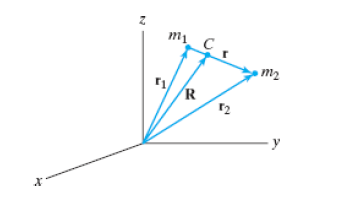
\includegraphics[width=0.4\textwidth]{Figures/6.1.png}
        \caption{质心位于$C$的双粒子系统}
        \label{fig:6.1}
    \end{figure}
    \begin{equation}
        \boxed{
            x = x_2 - x_1, \quad y = y_2 - y_1, \quad z = z_2 - z_1
        }
        \label{eq:6.28}
    \end{equation}
    $x$、$y$和$z$称为\textbf{相对坐标}或\textbf{内坐标}(relative or internal coordinates)。

    我们现在从原点指向系统的质心$C$画出矢量$\mathbf{R}$,其分量用$X$、$Y$和$Z$表示:
    \begin{equation}
        \mathbf{R} = \mathbf{i}X + \mathbf{j}Y + \mathbf{k}Z
        \label{eq:6.29}
    \end{equation}
    根据双粒子系统质心的定义,有
    \begin{equation}
        X = \frac{m_1x_1 + m_2x_2}{m_1 + m_2}, \quad Y = \frac{m_1y_1 + m_2y_2}{m_1 + m_2}, \quad Z = \frac{m_1z_1 + m_2z_2}{m_1 + m_2}
        \label{eq:6.30}
    \end{equation}
    这三个方程与矢量方程等价:
    \begin{equation}
        \mathbf{R} = \frac{m_1\mathbf{r}_1 + m_2\mathbf{r}_2}{m_1 + m_2}
        \label{eq:6.31}
    \end{equation}
    我们也有
    \begin{equation}
        \mathbf{r} = \mathbf{r}_2 - \mathbf{r}_1
        \label{eq:6.32}
    \end{equation}
    我们将式(\ref{eq:6.31})和(\ref{eq:6.32})联立为关于$\mathbf{r}_1$和$\mathbf{r}_2$的方程组,并求解得到
    \begin{equation}
        \mathbf{r}_1 = \mathbf{R} - \frac{m_2}{m_1 + m_2}\mathbf{r}, \quad \mathbf{r}_2 = \mathbf{R} + \frac{m_1}{m_1 + m_2}\mathbf{r}
        \label{eq:6.33}
    \end{equation}
    方程(\ref{eq:6.31})和(\ref{eq:6.32})代表了一种将$x_1,y_1,z_1$和$x_2,y_2,z_2$坐标转换为$X,Y,Z$和$x,y,z$坐标的变换。考虑一下在这种变化下,系统的哈密顿量会发生什么变化。用字母顶上的点表示对时间的导数。粒子1的速度为[式(\ref{eq:5.34})]$\mathbf{v}_1 = \mathrm{d}\mathbf{r}_1/\mathrm{d}t = \dot{\mathbf{r}}_1$。系统的动能为两个粒子的动能之和:
    \begin{equation}
        T = \frac{1}{2}m_1\left|\dot{\mathbf{r}_1}\right|^2 + \frac{1}{2}m_2\left|\dot{\mathbf{r}_2}\right|^2
        \label{eq:6.34}
    \end{equation}
    将(\ref{eq:6.33})的时间导数代入(\ref{eq:6.34}),我们得到
    \begin{equation*}
        \begin{aligned}
            T = & \frac{1}{2}m_1\left(\dot{\mathbf{R}} - \frac{m_2}{m_1+m_2}\dot{\mathbf{r}}\right)\cdot \left(\dot{\mathbf{R}} - \frac{m_2}{m_1+m_2}\dot{\mathbf{r}}\right) \\
            & + \frac{1}{2}m_2\left(\dot{\mathbf{R}} + \frac{m_1}{m_1+m_2}\dot{\mathbf{r}}\right)\cdot \left(\dot{\mathbf{R}} + \frac{m_1}{m_1+m_2}\dot{\mathbf{r}}\right) \\
        \end{aligned}
    \end{equation*}
    其中,我们用到了$\left|\mathbf{A}\right|^2 = \mathbf{A}\cdot \mathbf{A}$[式(\ref{eq:5.24})]。使用矢量数量积的分配律,化简后,我们得到
    \begin{equation}
        T = \frac{1}{2}\left(m_1 + m_2\right)\left|\dot{\mathbf{R}}\right|^2 + \frac{1}{2}\left(\frac{m_1m_2}{m_1+m_2}\right)\left|\dot{\mathbf{r}}\right|^2
        \label{eq:6.35}
    \end{equation}
    令$M$为系统的总质量:
    \begin{equation}
        M \equiv m_1 + m_2
        \label{eq:6.36}
    \end{equation}
    我们定义双粒子系统的\textbf{折合质量}(reduced mass)为
    \begin{equation}
        \boxed{
            \mu \equiv \frac{m_1m_2}{m_1+m_2}
        }
        \label{eq:6.37}
    \end{equation}
    那么
    \begin{equation}
        T = \frac{1}{2}M\left|\dot{\mathbf{R}}\right|^2 + \frac{1}{2}\mu\left|\dot{\mathbf{r}}\right|^2
        \label{eq:6.38}
    \end{equation}

    (\ref{eq:6.38})的第一项是质量为$M$的整个系统平动产生的动能。\textbf{平动}(translational motion)是指每个质点都经历相同位移的运动。$\frac{1}{2}M\left|\dot{\mathbf{R}}\right|^2$是位于质心,具有质量$M$的假想粒子的动能。(\ref{eq:6.38})的第二项是两个粒子内运动(相对运动)产生的动能。内运动有两种形式。两个粒子间的距离$r$可以变化(振动),以及矢量$\mathbf{r}$的方向可以发生变化(转动)。注意:$\left|\dot{\mathbf{r}}\right| = \left|\mathrm{d}\mathbf{r}/\mathrm{d}t\right| \neq \mathrm{d}\left|\mathbf{r}\right|/\mathrm{d}t$。

    与六个原始坐标$x_1,y_1,z_1,x_2,y_2,z_2$相对应,我们有六个线动量:
    \begin{equation}
        p_{x_1} = m_1\dot{x}_1, \quad \ldots, \quad p_{z_2} = m_2\dot{z}_2
        \label{eq:6.39}
    \end{equation}
    将(\ref{eq:6.34})和(\ref{eq:6.38})相比较,我们将新坐标$X,Y,Z,x,y,z$的动量定义为
    \begin{equation*}
        p_X \equiv M\dot{X}, \quad p_Y \equiv M\dot{Y}, \quad p_Z \equiv M\dot{Z}
    \end{equation*}
    \begin{equation*}
        p_x \equiv \mu\dot{x}, \quad p_y \equiv \mu\dot{y}, \quad p_z \equiv \mu\dot{z}
    \end{equation*}
    我们定义两个新动量矢量:
    \begin{equation*}
        \mathbf{p}_M = \mathbf{i}M\dot{X} + \mathbf{j}M\dot{Y} + \mathbf{k}M\dot{Z},
        \quad \text{和} \quad \mathbf{p}_{\mu} = \mathbf{i}\mu\dot{x} + \mathbf{j}\mu\dot{y} + \mathbf{k}\mu\dot{z}
    \end{equation*}
    将这些动量代入式(\ref{eq:6.38}),我们得到
    \begin{equation}
        T = \frac{\left|\mathbf{p}_M\right|^2}{2M} + \frac{\left|\mathbf{p}_{\mu}\right|^2}{2\mu}
        \label{eq:6.40}
    \end{equation}

    现在,我们来考虑势能。我们限制$V$只是两个粒子的相对坐标$x$、$y$和$z$的函数:
    \begin{equation}
        V = V\left(x,y,z\right)
        \label{eq:6.41}
    \end{equation}
    (\ref{eq:6.41})的一个例子是相互作用遵守库仑定律的两个带电粒子[见式(\ref{eq:3.53})]。根据对$V$的这一限制,哈密顿函数为
    \begin{equation}
        H = \frac{p_M^2}{2M} + \left[\frac{p_{\mu}^2}{2\mu} + V\left(x,y,z\right)\right]
        \label{eq:6.42}
    \end{equation}

    现在,假设我们有一个由质量为 $M$ 的粒子和质量为 $\mu$ 的粒子组成的系统,前者不受力,后者受势能函数 $V\left(x,y,z\right)$ 的作用。再假设这些粒子之间没有相互作用。如果$\left(X,Y,Z\right)$表示质量为$M$的粒子的坐标,而$\left(x,y,z\right)$表示质量为$\mu$的粒子的坐标,那么这个假设系统的哈密顿量是什么?显然,它与式(\ref{eq:6.42})完全相同。

    哈密顿量(\ref{eq:6.42})可以看作是两个无相互作用假想粒子的哈密顿量之和:质量为$M$的粒子其哈密顿量为$p_M^2/2M$,质量为$\mu$的粒子其哈密顿量为$p_{\mu}^2/2\mu + V\left(x,y,z\right)$。因此,第\ref{sec:6.2 Noninteracting Particles and Separation of Variables}的结果表明:系统的量子力学能量是两个假想粒子的能量之和[式(\ref{eq:6.23})]:$E = E_M + E_{\mu}$。由式(\ref{eq:6.24})和(\ref{eq:6.42})可知,平动能$E_M$可以通过求解薛定谔方程$\left(\hat{p}_M^2/2M\right)\psi_M = E_M\psi_M$得到。这是质量为$M$的自由粒子的薛定谔方程,因此其可能的本征值全是非负数[式(\ref{neq:2.31})]:$E_m \ge 0$。由式(\ref{eq:6.42})和(\ref{eq:6.24})可知,内运动能$E_{\mu}$可以通过求解以下薛定谔方程得到:
    \begin{equation}
        \left[\frac{\hat{p}_{\mu}^2}{2\mu} + V\left(x,y,z\right)\right]\psi_{\mu}\left(x,y,z\right) = E_{\mu}\psi_{\mu}\left(x,y,z\right)
        \label{eq:6.43}
    \end{equation}

    这样,我们就把两个粒子根据仅取决于相对坐标 $x$、$y$、$z$ 的势能函数 $V\left(x,y,z\right)$ 进行相互作用的问题分离成了两个独立的单粒子问题:(1)质量为$M$的整体系统平动,它只是在系统能量的基础上增加了一个恒非负的能量$E_M$;(2)通过求解质量为 $\mu$ 的假想粒子的薛定谔方程 (\ref{eq:6.43})来处理相对运动或内部运动,该粒子的坐标为相对坐标 $x$、$y$、$z$,并在势能 $V\left(x,y,z\right)$ 的作用下运动。

    例如,对于包含一个电子(e)和一个质子(p)的氢原子,原子的总能量为$E = E_M + E_{\mu}$,其中的$E_M$是质量为$M = m_e+m_p$的整个原子在空间中的平动能,其中的$E_{\mu}$是通过将$\mu = m_em_p/(m_e+m_p)$代入(\ref{eq:6.43})得到的,$V$ 是电子和质子相互作用的库仑定律势能;见第 \ref{sec:6.5 The Hydrogen Atom} 节。

\section{双粒子的刚性转子模型}
\label{sec:6.4 The Two-Particle Rigid Rotor}
    在求解氢原子的薛定谔方程之前,我们先来处理双粒子的刚性转子。这是一个双粒子系统,粒子之间的距离固定,由一根长度为$d$的刚性无质量杆连接。对于这个问题,图\ref{fig:6.1}中的矢量$\mathbf{r}$的长度$\left|\mathbf{r}\right|$是常数$d$。因此(见第\ref{sec:6.3 Reduction of the Two-Particle Problem to Two One-Particle Problems}节),内运动的动能完全是转动能。转子的能量完全由动能提供,以及
    \begin{equation}
        V=0
        \label{eq:6.44}
    \end{equation}
    方程(\ref{eq:6.44})是(\ref{eq:6.41})的一个特例,因此,我们可以利用上一节得到的结果,将系统的平动分离出来。我们将只关注转动能量。旋转运动的哈密顿算符由(\ref{eq:6.43})中括号内的项给出:
    \begin{equation}
        \hat{H} = \frac{\hat{p}_{\mu}^2}{2\mu} = -\frac{\hbar^2}{2\mu}\nabla^2, \quad \mu = \frac{m_1m_2}{m_1+m_2}
        \label{eq:6.45}
    \end{equation}
    其中$m_1$和$m_2$是两个粒子的质量。质量为$\mu$的假想粒子的坐标为$m_1$和$m_2$之间的相对坐标。[式(\ref{eq:6.28})]。

    与使用相对笛卡尔坐标$x$、$y$和$z$不同,使用相对球坐标$r$、$\theta$和$\phi$来描述转子会更有成效。$r$坐标与图\ref{fig:6.1}中的矢量$\mathbf{r}$的长度相同,由于$m_1$和$m_2$受限于保持固定的距离,我们有$r=d$。因此,这个问题等价于一个质量为$\mu$的粒子受限在半径为$r$的球面上运动。由于径向坐标是恒定的,波函数将只是$\theta$和$\phi$的函数。因此,对波函数进行运算时,式(\ref{eq:6.8})中拉普拉斯算符的前两项为零,可以省略。换个角度看问题,我们注意到式(\ref{eq:6.8})中涉及$r$导数的算符对应于径向运动的动能,而由于没有径向运动,$\hat{H}$中不包含$r$的导数。

    由于$V=0$是$V=V\left(r\right)$的特例,第\ref{sec:6.1 The One-Particle Central Force Problem}节的结论表明:本征函数由式(\ref{eq:6.16})给出,其中$r$的因子被省略:
    \begin{equation}
        \psi = Y_l^m\left(\theta, \phi\right)
        \label{eq:6.46}
    \end{equation}
    其中,转动角量子数用$J$而不是$l$来表示。

    哈密顿算符由式(\ref{eq:6.8})给出,其中省略了$r$的导数及$V\left(r\right) = 0$。因此,
    \begin{equation*}
        \hat{H} = \left(2\mu d^2\right)^{-1}\hat{L}^2
    \end{equation*}
    使用式(\ref{eq:6.13}),有
    \begin{equation*}
        \begin{aligned}
            \hat{H}\psi & = E\psi \\
            \left(2\mu d^2\right)^{-1}\hat{L}^2Y_J^m\left(\theta, \phi\right) & = EY_J^m\left(\theta, \phi\right) \\
            \left(2\mu d^2\right)^{-1}J\left(J+1\right)\hbar^2Y_J^m\left(\theta, \phi\right) & = EY_J^m\left(\theta, \phi\right) \\
        \end{aligned}
    \end{equation*}
    \begin{equation}
        E = \frac{J\left(J+1\right)\hbar^2}{2\mu d^2}
        \label{eq:6.47}
    \end{equation}

    由$n$个粒子组成的系统绕空间某一特定轴旋转产生的\textbf{转动惯量}(moment of inertia)$I$定义为
    \begin{equation}
        I \equiv \sum_{i=1}^{n}m_i\rho_i^2
        \label{eq:6.48}
    \end{equation}
    其中$m_i$是粒子$i$的质量,$\rho_i$是粒子$i$到旋转轴的垂直距离。$I$的值与选择的旋转轴有关。对于双粒子的刚性转子,我们选择通过质心并垂直于连接 $m_1$ 和 $m_2$ 的直线作为我们的轴线(图 \ref{fig:6.2})。如果我们将转子置于坐标系的$x$轴上,使得质心$C$位于原点,连接$m_1$和$m_2$的直线与$x$轴重合,那么$C$的坐标为$\left(0,0,0\right)$,$m_1$的坐标为$\left(-\rho_1,0,0\right)$,$m_2$的坐标为$\left(\rho_2,0,0\right)$。将这些坐标带入式(\ref{eq:6.30}),我们得到
    \begin{equation}
        m_1\rho_1 = m_2\rho_2
        \label{eq:6.49}
    \end{equation}
    \begin{figure}[ht]
        \centering
        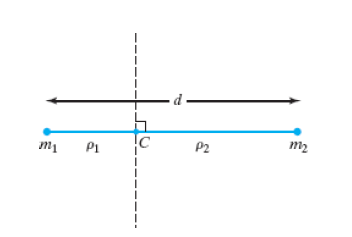
\includegraphics[width=0.4\textwidth]{Figures/6.2.png}
        \caption{
            \centering\parbox{\linewidth}{
                \centering
                用于计算双粒子刚性转子 \\
                转动惯量的轴线(虚线)。\\
                $C$是质心。
            }
        }
        \label{fig:6.2}
    \end{figure}
    转子绕我们选择的轴旋转的转动惯量为
    \begin{equation}
        I = m_1\rho_1^2 + m_2\rho_2^2
        \label{eq:6.50}
    \end{equation}
    使用式(\ref{eq:6.49}),我们可以将(\ref{eq:6.50})写成(问题6.14)
    \begin{equation}
        \boxed{
            I = \mu d^2
        }
        \label{eq:6.51}
    \end{equation}
    其中$\mu \equiv m_1m_2/(m_1+m_2)$是系统的折合质量,$d \equiv \rho_1 + \rho_2$是$m_1$和$m_2$之间的距离。双粒子刚性转子允许的能级由式(\ref{eq:6.47})给出:
    \begin{equation}
        \boxed{
            E = \frac{J\left(J+1\right)\hbar^2}{2I}, \quad J = 0, 1, 2, \ldots
        }
        \label{eq:6.52}
    \end{equation}
    最低的能级满足$E=0$,所以没有零点转动能。转动能为零,因此转子的角动量为零,这并不违反不确定性原理;回顾公式(\ref{eq:5.105})后面的讨论。请注意:$E$随着$J^2+J$的增大而增大,因此相邻旋转能级的间隔随着$J$的增大而增大。

    转子的能级(\ref{eq:6.52})是简并的吗?能量只取决于$J$,而波函数(\ref{eq:6.46})同时取决于$J$和$m$,其中$m\hbar$是转子角动量在$z$方向上的分量。对于每个$J$的值,都有$2J+1$个$m$的可能值,从$-J$到$J$。因此,能级是$\left(2J+1\right)$-重简并的。简并能级的状态具有不同的转子绕空间固定轴方向的角动量矢量方向。

    波函数(\ref{eq:6.46})中的$\theta$和$\phi$角是两个质点的相对坐标。如果我们建立一个笛卡尔坐标系,令转子的质心与原点重合,那么$\theta$和$\phi$将如图\ref{fig:6.3}所示。该坐标系与转子质心的平移运动相同,但不在空间中转动。

    转动角动量$\left[J\left(J+1\right)\hbar^2\right]^{1/2}$是两个粒子相对于系统质心$C$处原点的角动量。

    双原子分子的旋转能级可以用双粒子刚性转子模型(\ref{eq:6.52})来很好地近似。研究发现(\textit{Levine, Molecular Spectroscopy}, Section 4.4 ):当双原子分子吸收或发射辐射时,允许的纯转动跃迁由以下选律给出:
    \begin{equation}
        \Delta J = \pm 1
        \label{eq:6.53}
    \end{equation}
    此外,分子必须具有非零偶极矩,才能显示出纯转动光谱。\textit{纯转动跃迁}(pure rotational transition)是指只有转动量子数发生变化的跃迁。[振动-转动跃迁(第\ref{sec:4.3 Vibrations of Diatomic Molecules}节)涉及振动量子数和转动量子数的变化。]相邻较低旋转能级之间的能级间隔明显小于振动能级之间的能级间隔,纯转动光谱位于微波(或远红外)区域。因此,双原子分子纯转动光谱线的频率(近似值)为:
    \begin{equation}
        \nu = \frac{E_{J+1} - E_J}{h} = \frac{\left[\left(J+1\right)\left(J+2\right) - J\left(J+1\right)\right]\hbar^2}{8\pi^2 I} = 2\left(J+1\right)B
        \label{eq:6.54}
    \end{equation}
    \begin{equation}
        B \equiv h/8\pi^2 I, \quad J = 0, 1, 2, \ldots
        \label{eq:6.55}
    \end{equation}
    $B$称为分子的\textbf{转动常数}(rotational constant)。
    \begin{figure}[ht]
        \centering
        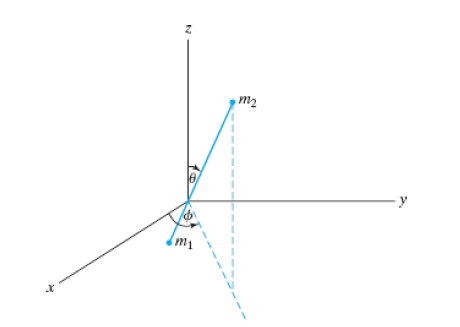
\includegraphics[width=0.4\textwidth]{Figures/6.3.png}
        \caption{双粒子刚性转子的坐标系}
        \label{fig:6.3}
    \end{figure}

    在室温下,具有较低$J$值的双粒子旋转能级间隔通常小于$kT$或与$kT$处于同一数量级,因此,玻尔兹曼分布律(\ref{eq:4.63})表明:室温下许多转动能级可以被显著占据。$J=0$的双原子分子吸收辐射后会产生一条频率为$2B$的谱线(对应$J = 0 \to 1$的跃迁),$J=1$的分子吸收辐射后会产生一条频率为$4B$的谱线(对应$J = 1 \to 2$的跃迁),$J=2$的分子吸收辐射后会产生一条频率为$6B$的谱线(对应$J = 2 \to 3$的跃迁),依此类推。见图\ref{fig:6.4}。
    \begin{figure}[ht]
        \centering
        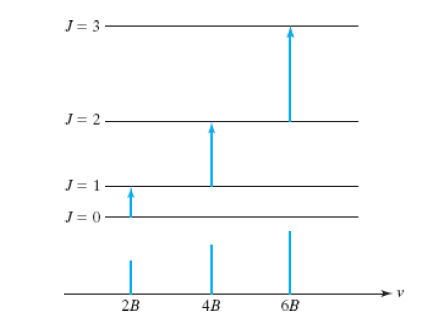
\includegraphics[width=0.4\textwidth]{Figures/6.4.png}
        \caption{双粒子刚性转子吸收跃迁}
        \label{fig:6.4}
    \end{figure}

    通过测量转动吸收频率可以得到$B$的值。根据$B$,我们可以得到分子的转动惯量$I$,根据$I$我们可以得到键长$d$。找到的$d$值是$v=0$振动运动的平均值。由于图\ref{fig:4.6}和图13.1中的势能曲线不对称,$d$比图13.1中的平衡键长略长。
    % 此处记得改引用!!!!!

    如第\ref{sec:4.3 Vibrations of Diatomic Molecules}节所述,$^1\mathrm{H}^{35}\mathrm{Cl}$和$^1\mathrm{H}^{37}\mathrm{Cl}$等同位素分子的电子能量曲线$U\left(R\right)$几乎相同,因此其平衡核间距也几乎相同。然而,不同的同位素质量会产生不同的转动惯量,从而产生不同的转动吸收频率。

    由于分子不是刚性的,因此双原子分子的旋转能级与刚性转子的旋转能级略有不同。由式(\ref{eq:6.52})和(\ref{eq:6.55}),双粒子刚性转子的能级为$E_{rot} = BhJ\left(J+1\right)$。由于分子振动的非谐性(图\ref{fig:4.6}、\ref{fig:4.5}),当振动量子数$v$增加时,核间距平均值也会增加,所以$v$增加时,转动惯量$I$也会增加,则转动常数$B$减小。为了考虑$B$对$v$的依赖性,在$E_{rot}$中用$B_v$代替$B$。振动能级$v$的\textit{平均转动常数}(mean rotational constant)$B_v$满足$B_v = B_e - \alpha_e\left(v+1/2\right)$,其中$B_e$是利用图\ref{fig:4.5}和\ref{fig:4.5}势能曲线底部的平衡核间距$R_e$计算得出的,\textit{振转耦合常数}(vibrational-rotational coupling constant)$\alpha_e$是一个大于零的常数(因分子的不同而异),且远小于$B_e$。此外,随着转动能量的增加,平衡核间距有非常轻微的增加[这种现象称为\textit{离心形变}(centrifugal distortion)]。这就在$E_{rot}$中引入了一项$-hDJ^2\left(J+1\right)^2$,其中离心形变常数$D$是一个极小的正数,随着分子的不同而异。例如,对$^{12}\mathrm{C}^{15}\mathrm{O}$分子,$B_0 = 57636 \: \mathrm{MHz}$,$\alpha_e = 540 \: \mathrm{MHz}$,$D = 0.18 \: \mathrm{MHz}$。如第\ref{sec:4.3 Vibrations of Diatomic Molecules}节所述,对于轻双原子分子,几乎所有分子在室温下都处在基态振动能级,观测到的转动常数为$B_0$。

    有关双原子分子核运动的更多讨论,请参见第\ref{sec:13.2 Nuclear Motion in Diatomic Molecules}节。关于多原子分子的转动能,请参见\textit{Townes and Schawlow}, chaps. 2-4。

    \begin{examplebox}
        \textbf{例题:}分子$^{12}\mathrm{C}^{32}\mathrm{S}$的最低频率纯转动吸收线位于$48991.0 \: \mathrm{MHz}$。计算分子的键长。
        \\
        \\
        最低频率的转动吸收为$J = 0 \to 1$线。根据式(\ref{eq:1.4 Higher state to lower state delta energy})、(\ref{eq:6.52})和(\ref{eq:6.51}),有
        \begin{equation*}
            h\nu = E_{upper} - E_{lower} = \frac{1\left(2\right)\hbar^2}{2\mu d^2} - \frac{0\left(1\right)\hbar^2}{2\mu d^2}
        \end{equation*}
        其中$d = \left(h/4\pi^2\nu\mu\right)^{1/2}$。使用附录中的表A.3,有
        \begin{equation*}
            \mu = \frac{m_1m_2}{m_1 + m_2} = \frac{12\left(31.97207\right)}{\left(12+31.97207\right)}\frac{1}{6.02214\times 10^{23}} \: \mathrm{g} = 1.44885 \times 10^{-23} \: \mathrm{kg}
        \end{equation*}
        质量的国际单位为千克,则
        \begin{equation*}
            \begin{aligned}
                d = \frac{1}{2\pi}\left(\frac{h}{\nu_{0 \to 1}\mu}\right)^{1/2} & = \frac{1}{2\pi}\left[\frac{6.62607 \times 10^{-34} \: \mathrm{J \cdot s}}{\left(48991.0 \times 10^6\: \mathrm{s}^{-1}\right) \left(1.44885 \times 10^{-26} \: \mathrm{kg}\right)}\right]^{1/2} \\
                & = 1.5377 \times 10^{-10} \: \mathrm{m} = 1.5377 \: \mathrm{Å}
            \end{aligned}
        \end{equation*}
        \\
        \\
        \textbf{练习:}分子$^{12}\mathrm{C}^{16}\mathrm{O}$的$J = 1 \to 2$的纯转动跃迁位于$230.538 \: \mathrm{GHz}$。(1 GHz = $10^9$ Hz。)计算分子的键长。(\textit{答案:}$1.1309 \times 10^{-10} \: \mathrm{m}$。)
    \end{examplebox}

\section{氢原子}
\label{sec:6.5 The Hydrogen Atom}
    氢原子包含一个质子和一个电子,若用$\mathrm{e}$表示质子的电荷量($\mathrm{e} = + 1.6 \times 10^{-19} \: \mathrm{C}$),则电子的电荷量为$-\mathrm{e}$。
    \begin{quote}
        \small
        一些科学家推测,质子和电子的电荷量并不完全相等。实验表明,电子和质子的电荷量差距在$10^{-21}$的数量级。见G. Bressi 等., \textit{Phys. Rev. A}, \textbf{83}, 052101 (2011) (available online at arxiv.org/abs/1102.2766).
    \end{quote}

    我们将假定质子和电子是质点,其相互作用遵守库仑定律。在讨论原子和分子时,我们通常会考虑孤立的系统,而忽略原子和分子间的相互作用。

    我们不只讨论氢原子,而是稍微考虑一个更为普遍的问题:\textbf{类氢原子}(hydrogenlike atom),它由一个电子和一个电荷为$Z\mathrm{e}$的原子核组成。若$Z=1$,则类氢原子就是氢原子;若$Z=2$,则类氢原子是\ce{He^+};若$Z=3$,则类氢原子是\ce{Li^{2+}};依此类推。类氢原子是量子化学中最重要的系统。由于存在电子间斥力,因此无法获得具有一个以上电子的原子的薛定谔方程的精确解。如果作为粗略的第一近似值,我们忽略这些斥力,那么电子就可以独立处理(参见第\ref{sec:6.2 Noninteracting Particles and Separation of Variables}节)。原子波函数将由单电子函数的乘积近似得出,而单电子函数将是类氢波函数。单电子波函数(无论是否为类氢波函数)称为\textbf{轨道}(orbital)。(更确切地说,\textbf{轨道}是一个单电子空间波函数,空间一词的意思是波函数取决于电子的三个空间坐标 $x$、$y$ 和 $z$ 或 $r$、$\theta$ 和 $\phi$。我们将在第 \ref{chap:10} 章中看到,电子自旋的存在为单电子波函数增加了第四个坐标,即所谓的自旋轨道。)原子中电子的轨道称为\textbf{原子轨道}(atomic orbital)。我们将使用原子轨道来构建多电子原子的近似波函数(第 \ref{chap:11} 章)。轨道还可用于构建分子的近似波函数。

    对于类氢原子,令$\left(x,y,z\right)$为电子相对于原子核的坐标,再令$\mathbf{r} = \mathbf{i}x+\mathbf{j}y+\mathbf{k}z$。电子在类氢原子中受到的库仑力为 [见公式 (\ref{eq:1.37 coulomb's law}) ]
    \begin{equation}
        \mathbf{F} = -\frac{Z\mathrm{e}^2}{4\pi\varepsilon_0r^2}\frac{\mathbf{r}}{r}
        \label{eq:6.56}
    \end{equation}
    其中$\mathbf{r}/r$是$\mathbf{r}$方向的单位矢量。负号表示为吸引力。

    \begin{quote}
        \small
        我们考虑了库仑定律出现微小偏差的可能性。实验表明,如果将库仑定律力写成与 $r^{-2+s}$ 成正比,那么 $\left|s\right|<10^{-16}$。库仑定律的偏差可以证明光子静止质量不为零。没有证据表明光子的静止质量不为零,而且数据表明,任何这种质量都必须小于 $10^{-51} \: \mathrm{g}$;A. S. Goldhaber and M. M. Nieto, \textit{Rev. Mod. Phys.}, \textbf{82}, 939 (2010) (arxiv.org/abs/0809.1003); G. Spavieri et al., \textit{Eur. Phys. J. D}, \textbf{61}, 531 (2011) (\url{link.springer.com/content/pdf/10.1140/epjd/e2011-10508-7}).
    \end{quote}

    式(\ref{eq:6.56})中的力是中心力,将其与式(\ref{eq:6.4})相比较,有$\mathrm{d}\left(r\right)/\mathrm{d}r = Z\mathrm{e}^2/4\pi\varepsilon_0r^2$。积分,得出
    \begin{equation}
        V = \frac{Z\mathrm{e}^2}{4\pi\varepsilon_0}\int\frac{1}{r^2}\mathrm{d}r = -\frac{Z\mathrm{e}^2}{4\pi\varepsilon_0r}
        \label{eq:6.57}
    \end{equation}
    其中积分常数取 0,以便在电荷间距无限大时能满足$V=0$。对于任意两个相距$r_{12}$,电荷量分别为$Q_1$和$Q_2$的粒子,式(\ref{eq:6.57})可以写成
    \begin{equation}
        \boxed{
            V = -\frac{Q_1Q_2}{4\pi\varepsilon_0r_{12}}
        }
        \label{eq:6.58}
    \end{equation}

    由于这个双粒子系统的势能只取决于粒子的相对坐标,我们可以应用第 \ref{sec:6.3 Reduction of the Two-Particle Problem to Two One-Particle Problems} 节的结果将问题简化为两个单粒子问题。原子的整体平移运动只是在总能量中增加了一个常数,我们将不再关注它。为了处理系统的内部运动,我们引入一个质量由下式定义的假想粒子
    \begin{equation}
        \mu = \frac{m_{\mathrm{e}}m_N}{m_{\mathrm{e}} + m_N}
        \label{eq:6.59}
    \end{equation}

   其中$m_{\mathrm{e}}$为电子的质量,$m_N$为原子核的质量。质量为 $\mu$ 的粒子在势能函数 (\ref{eq:6.57}) 的作用下运动,其坐标$\left(r,\theta,\phi\right)$是一个粒子相对于另一个粒子的球面坐标(图\ref{fig:6.5})。
   \begin{figure}
       \centering
       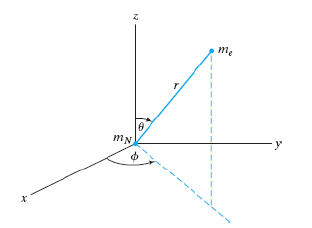
\includegraphics[width=0.5\textwidth]{Figures/6.5.png}
       \caption{相对球坐标}
       \label{fig:6.5}
   \end{figure}

   粒子内部运动的哈密顿算符为[式(\ref{eq:6.43})]
   \begin{equation}
        \hat{H} = -\frac{\hbar^2}{2\mu}\nabla^2 - \frac{Z\mathrm{e}^2}{4\pi\varepsilon_0r}
        \label{eq:6.60}
   \end{equation}
   由于$V$只是坐标$r$的函数,这是一个单粒子中心力问题,所以我们可以使用第\ref{sec:6.1 The One-Particle Central Force Problem}节的结果来求解。使用方程(\ref{eq:6.16})和(\ref{eq:6.17}),我们可以写出波函数
   \begin{equation}
        \psi\left(r,\theta,\phi\right) = R\left(r\right)Y_l^m\left(\theta,\phi\right), \quad l = 0, 1, 2, \ldots, \quad \left|m\right| \leq l
    \label{eq:6.61}
   \end{equation}
   其中$Y_l^m$是球谐函数,径向函数$R\left(r\right)$满足
   \begin{equation}
        -\frac{\hbar^2}{2\mu}\left(R^{\prime\prime} + \frac{2}{r}R^{\prime}\right) + \frac{l\left(l+1\right)\hbar^2}{2\mu r^2}R - \frac{Z\mathrm{e}^2}{4\pi\varepsilon_0r}R = ER\left(r\right)
        \label{eq:6.62}
   \end{equation}
   为了节省时间,我们定义常数$a$满足
   \begin{equation}
        a \equiv \frac{4\pi\varepsilon_0\hbar^2}{\mu \mathrm{e}^2}
        \label{eq:6.63}
   \end{equation}
   则方程(\ref{eq:6.62})可以写成
   \begin{equation}
        R^{\prime\prime} + \frac{2}{r}R^{\prime} + \left[\frac{8\pi\varepsilon_0E}{a\mathrm{e}^2} + \frac{2Z}{ar} - \frac{l\left(l+1\right)}{r^2}\right]R = 0
        \label{eq:6.64}
   \end{equation}

\subsection*{径向方程的求解}
   现在我们可以尝试 (\ref{eq:6.64}) 的幂级数解法,但得到的是三项递推关系,而不是两项递推关系。因此,我们要寻找一种能得到两项递推关系的替代方法。事实证明,通过研究大 $r$ 值时解的行为,可以找到合适的替代方法。当$r$值很大时,方程(\ref{eq:6.64})变为
   \begin{equation}
        R^{\prime\prime} + \frac{8\pi\varepsilon_0E}{a\mathrm{e}^2}R = 0, \quad \text{当}r\text{很大时}
        \label{eq:6.65}
   \end{equation}
   该微分方程可以使用特征方程(\ref{eq:2.7 auxiliary equation})求解。其解为
   \begin{equation}
        \exp\left[\pm\left(-8\pi\varepsilon_0E/a\mathrm{e}^2\right)^{1/2}r\right]
        \label{eq:6.66}
   \end{equation}

   假设 $E$ 为正数。(\ref{eq:6.66}) 中平方根符号下的量是负数,乘以 $r$ 的因子是虚数:
   \begin{equation}
        R\left(r\right) \sim \mathrm{e}^{\pm \mathrm{i}\sqrt{2\mu Er}/\hbar}, \quad E \geq 0
        \label{eq:6.67}
   \end{equation}
   其中我们用到了(\ref{eq:6.63})。(\ref{eq:6.67})中的符号$\sim$表示我们给出的是在$r$值较大时$R\left(r\right)$的行为,这就是函数的\textit{渐近}(asymptotic)行为。请注意 (\ref{eq:6.67}) 与自由粒子波函数公式 (\ref{eq:2.30}) 的相似性。 (\ref{eq:6.67}) 并没有给出正能量波函数中的完整径向因子。进一步的研究(\textit{Bethe and Salpeter},第 21-24 页)表明,无论 $E$ 的值如何,$E \geq 0$ 的径向函数在所有 $r$ 值上都是有限的。因此,正如自由粒子一样,氢原子的所有非负能量都是允许的。在物理学上,这些本征函数对应于电子不与原子核结合的状态,即原子电离时的状态。(一个经典的机械比喻是彗星围绕太阳在双曲线轨道上运动。彗星不受约束,只访问太阳系一次。)由于我们得到的 $E \geq 0$ 的允许值是连续的而不是离散的,因此正能量本征函数又称为\textbf{连续谱本征函数}(continuum eigenfunctions)。连续谱波函数的角度部分是球面谐波。与自由粒子波函数一样,连续谱本征函数也不是通常意义上可归一化的。

   现在我们考虑氢原子的\textit{束缚}态,即 $E < 0$。(对于一个\textbf{束缚态},当$x \to \pm \infty$时,$\psi \to 0$。)在这种情况下,(\ref{eq:6.66})中括号内的量为正数。由于我们希望波函数在 $r$ 变为无穷大时保持有限,因此我们更倾向于使用 (\ref{eq:6.66}) 中的负号,为了得到两项递推关系,我们将其替换为
   \begin{equation}
        R\left(r\right) = \mathrm{e}^{-Cr}K\left(r\right)
        \label{eq:6.68}
   \end{equation}
   \begin{equation}
        C \equiv \left(-\frac{8\pi\varepsilon_0E}{a\mathrm{e}^2}\right)^{1/2}
        \label{eq:6.69}
   \end{equation}
   其中,(\ref{eq:6.68})中的$\mathrm{e}$是自然对数的底数,而不是电子的电荷量。使用代换 (\ref{eq:6.68}) 无法保证当$r$很大时的波函数行为。这样代换得到的微分方程仍然有两个线性独立的解。我们可以在微分方程中进行任意代换;事实上,我们可以进行如下代换$R\left(r\right) = \mathrm{e}^{+Cr}J\left(r\right)$并最终得到正确的本征函数和本征值。$J$和$K$的关系自然是$J\left(r\right) = \mathrm{e}^{-2Cr}K\left(r\right)$。

   根据(\ref{eq:6.68}),我们来计算$R^{\prime}$和$R^{\prime\prime}$,带入(\ref{eq:6.64}),乘以$r^2\mathrm{e}^{Cr}$并利用(\ref{eq:6.69})得到$K\left(r\right)$的微分方程:
   \begin{equation}
        r^2K^{\prime\prime} + \left(2r - 2Cr^2\right)K^{\prime} + \left[\left(2Za^{-1} - 2C\right)r - l\left(l+1\right)\right]K = 0
        \label{eq:6.70}
   \end{equation}

   现在,我们可以用以下形式的幂级数来代替$K$:
   \begin{equation}
        K = \sum_{k=0}^{\infty}c_kr^k
        \label{eq:6.71}
   \end{equation}
   如果我们这样做,就会发现:一般来说,(\ref{eq:6.71})中的前几项的系数都是零。如果$c_s$是第一个不为零的系数,那么(\ref{eq:6.71})可以写为
   \begin{equation}
        K = \sum_{s}^{\infty}c_kr^k, \quad c_s \neq 0
        \label{eq:6.72}
   \end{equation}
   令$j \equiv k-s$,再定义$b_j \equiv c_{j+s}$,我们有
   \begin{equation}
        K = \sum_{j=0}^{\infty}c_{j+s}r^{j+s} = r^s\sum_{j=0}^{\infty}b_jr^j, \quad b_0 \neq 0
        \label{eq:6.73}
   \end{equation}
   (虽然我们所做的各种替换看似随意,但它们却是用幂级数求解微分方程的标准程序。)将整数 $s$ 代入微分方程即可求出结果。方程(\ref{eq:6.73})变为
   \begin{equation}
        K\left(r\right) = r^sM\left(r\right)
        \label{eq:6.74}
   \end{equation}
   \begin{equation}
        M\left(r\right) = \sum_{j=0}^{\infty}b_jr^j, \quad b_0 \neq 0
        \label{eq:6.75}
   \end{equation}
   求出(\ref{eq:6.74})中的$K^{\prime}$和$K^{\prime\prime}$,将其代入(\ref{eq:6.70}),得到
   \begin{equation}
        r^2M^{\prime\prime} + \left[\left(2s+2\right)r - 2Cr^2\right]M^{\prime} + \left[s^2 + s + \left(2Za^{-1} - 2C -2Cs\right)r - l\left(l+1\right)\right]M = 0
        \label{eq:6.76}
   \end{equation}

   为了求出$s$,我们先看$r=0$时的(\ref{eq:6.76})。由(\ref{eq:6.75}),我们得到
   \begin{equation}
        M\left(0\right) = b_0, \quad M^{\prime}\left(0\right) = b_1, \quad M^{\prime\prime}\left(0\right) = 2b_2
        \label{eq:6.77}
   \end{equation}
   在(\ref{eq:6.76})中使用(\ref{eq:6.77}),得到
   \begin{equation}
        b_0\left(s^2+s-l^2-l\right) = 0
        \label{eq:6.78}
   \end{equation}
   由于$b_0$不为零,括号中式子就必须为零:$s^2+s-l^2-l=0$。这是一个关于未知数$s$的二次方程。它的根为
   \begin{equation}
        s = l, \quad s = -l-1
        \label{eq:6.79}
    \end{equation}
    这些根对应于微分方程的两个线性独立解。让我们从波函数正确行为的角度来研究它们。由(\ref{eq:6.68})、(\ref{eq:6.74})和(\ref{eq:6.75}),我们有
    \begin{equation}
        R\left(r\right) = \mathrm{e}^{-Cr}r^s\sum_{j=0}^{\infty}b_jr^j
        \label{eq:6.80}
    \end{equation}
    由于$\mathrm{e}^{-Cr} = 1-Cr+\ldots$,当$r$很小时,$R\left(r\right)$的行为与$b_0r^s$相同。当$s=l$时,$R\left(r\right)$在原点处表现正常。然而,当$s = -l-1$时,$R\left(r\right)$与下式在$r$很小时成正比:
    \begin{equation}
        \frac{1}{r^{l+1}}
        \label{eq:6.81}
    \end{equation}
    由于$l=0,1,2,\ldots$,则根$s=-l-1$使得波函数中径向部分在原点处变得无限大。许多文献都将此作为拒绝接受这一根的充分理由。然而,这并不是一个很好的论据,因为对于\textit{相对论}(relativistic)氢原子来说,$l=0$的本征函数在$r=0$处是无限的。因此,让我们从平方可积性的角度来研究 (\ref{eq:6.81}),因为我们当然要求束缚态本征函数是可归一化的。

    与 (\ref{eq:6.81}) 类似的径向函数的归一化积分[式 (\ref{eq:5.80}) ] (当$r$不是很大时)如下
    \begin{equation}
        \int_{0}\left|R\right|^2r^2\mathrm{d}r \approx \int_{0}\frac{1}{r^{2l}}\mathrm{d}r
        \label{eq:6.82}
    \end{equation}
    积分下限处的积分行为是
    \begin{equation}
        \left.\frac{1}{r^{2l}}\right|_{r=0}
        \label{eq:6.83}
    \end{equation}
    对于$l=1,2,3,\ldots$,(\ref{eq:6.83})是无限的,那么归一化积分也是无限的。因此我们舍去当$l \geq 1$时的根$s = -l-1$。不过,对于 $l=0$,(\ref{eq:6.83}) 是有限的,平方可积性也没有问题。因此,径向方程存在一个平方可积的解,在小 $r$ 时表现为 $r^{-1}$ 。

    对这一解决方案的进一步研究表明,它所对应的能量值是实验氢原子谱所不存在的。因此,$r^{-1}$的解必须被舍去,但对这样做的原因存在一些争议。一种观点认为:除原点外,$1/r$ 的在空间的任何地方都满足薛定谔方程,因此必须予以舍去[\textit{Dirac}, page 156; B. H. Armstrong and E. A. Power, \textit{Am. J. Phys.}, \textbf{31}, 262 (1963)]。第二种观点认为,必须舍去 $1/r$ 的解,因为哈密顿算符对它来说不是厄米的(\textit{Merzbacher}, Section 10.5)。(在第 \ref{chap:7} 章中,我们将定义厄米算符,并说明量子力学算符必须是厄米的。)进一步讨论见 A. A. Khelashvili 和 T. P. Nadareishvili, \textit{Am. J. Phys.}, \textbf{79}, 668 (2011) (see arxiv.org/abs/1102.1185) and in Y. C. Cantelaube, arxiv.org/abs/1203.0551.

    取(\ref{eq:6.79})的第一个根,我们得到了径向部分的因子(\ref{eq:6.80})
    \begin{equation}
        R\left(r\right) = \mathrm{e}^{-Cr}r^lM\left(r\right)
        \label{eq:6.84}
    \end{equation}
    由于$s=l$,(\ref{eq:6.75})变为
    \begin{equation}
        rM^{\prime\prime} + \left(2l+1-2Cr\right)M^{\prime} + \left(2Za^{-1}-2C-2Cl\right)M = 0
        \label{eq:6.85}
    \end{equation}
    由(\ref{eq:6.75}),我们有
    \begin{equation}
        M\left(r\right) = \sum_{j=0}^{\infty}b_jr^j
        \label{eq:6.86}
    \end{equation}
    \begin{equation*}
        M^{\prime} = \sum_{j=0}^{\infty}b_jjr^{j-1} = \sum_{j=1}^{\infty}jb_jr^{j-1} = \sum_{k=0}^{\infty}\left(k+1\right)b_{k+1}r^k = \sum_{j=0}^{\infty}\left(j+1\right)b_{j+1}r^j
    \end{equation*}
    \begin{equation*}
        M^{\prime\prime} = \sum_{j=0}^{\infty}j\left(j-1\right)b_jr^{j-2} = \sum_{j=1}^{\infty}b_jj\left(j-1\right)r^{j-2} = \sum_{k=0}^{\infty}\left(k+1\right)kb_{k+1}r^{k-1}
    \end{equation*}
    \begin{equation}
        M^{\prime\prime} = \sum_{j=0}^{\infty}\left(j+1\right)jb_{j+1}r^{j-1}
        \label{eq:6.87}
    \end{equation}
    将这些式子带入(\ref{eq:6.85})并求和,得到
    \begin{equation*}
        \sum_{j=0}^{\infty}\left[j\left(j+1\right)b_{j+1} + 2\left(l+1\right)\left(j+1\right)b_{j+1} + \left(\frac{2Z}{a} - 2C - 2Cl - 2Cj\right)b_j\right]r^j = 0
    \end{equation*}
    令$r^j$的系数为零,得到递推关系式
    \begin{equation}
        b_{j+1} = \frac{2C + 2Cl + 2Cj - 2Za^{-1}}{j\left(j+1\right) + 2\left(l+1\right)\left(j+1\right)}b_j
        \label{eq:6.88}
    \end{equation}

    现在我们必须研究大 $r$ 时无穷级数 (\ref{eq:6.86}) 的行为。根据对 (\ref{eq:4.42}) 中谐振子幂级数的相同检验方法得出的结果,对于大 $r$,无穷级数 (\ref{eq:6.86}) 的表现与$\mathrm{e}^{2Cr}$一致(见问题6.20)。当$r$很大时,径向函数(\ref{eq:6.84})的表现为
    \begin{equation}
        R\left(r\right) \sim \mathrm{e}^{-Cr}r^l\mathrm{e}^{2Cr} = r^l\mathrm{e}^{Cr}
        \label{eq:6.89}
    \end{equation}
    因此,当$r$变得无穷大时,$R\left(r\right)$将变为无穷大,并且不具有平方可积性。避免这种 “无穷大灾难”(如谐振子情况)的唯一方法是让级数在有限的项数后被打断,在这种情况下,$\mathrm{e}^{-Cr}$ 因子将确保波函数在 $r$ 变为无穷大时趋于零。令该级数的最后一项为$b_kr^k$。那么为了使$b_{k+1}, b_{k+2}, \ldots$ 都为零,我们必须让 $j=k$ 时,递推关系 (\ref{eq:6.88}) 中与 $b_j$ 相乘的系数消失。因此,
    \begin{equation}
        2C\left(k+l+1\right) = 2Za^{-1}, \quad k = 0, 1, 2, \ldots
        \label{eq:6.90}
    \end{equation}
    $k$和$l$都是整数,现在我们定义一个新的整数$n$:
    \begin{equation}
        n \equiv k + l + 1, \quad n = 1, 2, 3, \ldots
        \label{eq:6.91}
    \end{equation}
    根据(\ref{eq:6.91}),量子数$l$必须满足
    \begin{equation}
        l \leq n-1
        \label{eq:6.92}
    \end{equation}
    因此,$l$的取值范围为0到$n-1$。
    \\

\subsubsection*{能级}

    将(\ref{eq:6.91})代入(\ref{eq:6.90}),得到
    \begin{equation}
        Cn = Za^{-1}
        \label{eq:6.93}
    \end{equation}
    将$C \equiv \left(-8\pi\varepsilon_0E/a\mathrm{e}^2\right)^{1/2}$[式(\ref{eq:6.69})]代入(\ref{eq:6.93}),解出$E$,得到
    \begin{equation}
        E = -\frac{Z^2}{n^2}\frac{\mathrm{e}^2}{8\pi\varepsilon_0a} = -\frac{Z^2\mu\mathrm{e}^4}{8\varepsilon_0^2n^2h^2}
        \label{eq:6.94}
    \end{equation}
    其中$a \equiv 4\pi\varepsilon_0\hbar^2/\mu\mathrm{e}^2$ [式(\ref{eq:6.63})]。这些是类氢原子的束缚态能级,它们是离散的。图 \ref{fig:6.6} 显示了氢原子($Z=1$)的势能曲线[公式 (\ref{eq:6.57}) ] 和一些允许能级。横线表示允许使用所有正能量。
    \begin{figure}
        \centering
        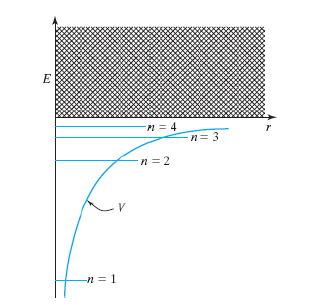
\includegraphics[width=0.5\textwidth]{Figures/6.6.png}
        \caption{氢原子的能级}
        \label{fig:6.6}
    \end{figure}

    事实证明,在光的吸收和发射过程中,$n$ 的所有变化都是允许的。因此,氢原子谱线的波长[公式 (\ref{eq:4.64}) ] 为
    \begin{equation}
        \tilde{\nu} = \frac{1}{\lambda} = \frac{\nu}{c} = \frac{E_2 - E_1}{hc} = \frac{\mathrm{e}^2}{8\pi\varepsilon_0ahc}\left(\frac{1}{n_1^2} - \frac{1}{n_2^2}\right) = R_H\left(\frac{1}{n_1^2} - \frac{1}{n_2^2}\right)
        \label{eq:6.95}
    \end{equation}
    其中$R_H = 109677.6 \: \mathrm{cm}^{-1}$是氢的\textit{里德伯常数}(Rydberg constant)。
    \\

\subsubsection*{简并}

    氢原子的能级是简并的吗?对于束缚态,能量(\ref{eq:6.94})只取决于 $n$。然而,波函数 (\ref{eq:6.61}) 取决于所有三个量子数 $n$、$l$ 和 $m$,它们的允许值分别为[式 (\ref{eq:6.91}) 、 (\ref{eq:6.92})、 (\ref{eq:5.104})  和 (\ref{eq:5.105}) ]
    \begin{equation}
        \boxed{
            n = 1,2,3,\ldots
        }
        \label{eq:6.96}
    \end{equation}
    \begin{equation}
        \boxed{
            l = 0,1,2,\ldots,n-1
        }
        \label{eq:6.97}
    \end{equation}
    \begin{equation}
        \boxed{
            m = -l,-l+1,\ldots,0,\ldots,l-1,l
        }
        \label{eq:6.98}
    \end{equation}
    $l$ 或 $m$ 值不同但 $n$ 值相同的氢原子态具有相同的能量。能级是简并的,只有 $n=1$ 除外,此时 $l$ 和 $m$ 必须都为 0。对于给定的 $n$ 值,我们可以有 $n$ 个不同的 $l$ 值。对于每个 $l$ 值,我们都可以有 $2l+1$ 个 $m$ 值。 H 原子束缚态能级的简并度等于$n^2$(省略了旋转方面的考虑),见问题6.16。对于连续能级,事实证明,对于给定的能量,$l$ 的最大值没有限制;因此,这些能级是无穷重简并的。

    氢原子的径向方程也可以通过梯形算符(也称为\textit{因式分解}(factorization))来求解;参见 Z. W. Salsburg, \textit{Am. J. Phys.}, \textbf{33}, 36 (1965)。

\section{束缚态氢原子波函数}
\label{sec:6.6 The Bound-State Hydrogen-Atom Wave Functions}

\subsection*{径向因子}
    使用(\ref{eq:6.93}),我们有递推关系(\ref{eq:6.88})
    \begin{equation}
        b_{j+1} = \frac{2Z}{na} = \frac{j+l+1-n}{\left(j+1\right)\left(j+2l+2\right)}b_j
        \label{eq:6.99}
    \end{equation}
    (\ref{eq:6.91})前面的讨论表明:多项式$M\left(r\right) = \sum_{j}b_jr^j$中$r$的最高次幂为$k = n-l-1$。因此,将$C = Z/na$(\ref{eq:6.93})代入$R\left(r\right) \mathrm{e}^{-Cr}r^lM\left(r\right)$(\ref{eq:6.84}),我们得到
    \begin{equation}
        R_{nl}\left(r\right) = r^l\mathrm{e}^{-Zr/na}\sum_{j=0}^{n-l-1}b_jr^j
        \label{eq:6.100}
    \end{equation}
    其中$a \equiv 4\pi\varepsilon_0\hbar^2/\mu\mathrm{e}^2$ [式(\ref{eq:6.63})]。完整的类氢束缚态波函数为[式 (\ref{eq:6.61}) ]
    \begin{equation}
        \psi_{nlm} = R_{nl}\left(r\right)Y_l^m\left(\theta,\phi\right) = R_{nl}\left(r\right)S_{lm}\left(\theta\right)\frac{1}{\sqrt{2\pi}}\mathrm{e}^{\mathrm{i}m\phi}
        \label{eq:6.101}
    \end{equation}
    其中前几个 $\theta$ 函数见表 \ref{tab:5.1}。

    $R\left(r\right)$有多少个节点?径向函数在$r = \infty$、$l \neq 0$时$r = 0$和使$M\left(r\right)$消失的$r$值处为零。$M\left(r\right)$是一个$n-l-1$次多项式,可以证明,$M\left(r\right) = 0$的所有根均为正实数。因此,除了原点和无穷远之外,$R\left(r\right)$还有$n-l-1$个节点。球谐函数的节点将在问题6.41中讨论。

\subsection*{基态波函数和能量}
    对于类氢原子的基态,我们有$n=1$, $l=0$,$m=0$。因此,径向因子(\ref{eq:6.100})为
    \begin{equation}
        R_{10}\left(r\right) = b_0\mathrm{e}^{-Zr/a}
        \label{eq:6.102}
    \end{equation}
    常数$b_0$可以通过归一化条件[式(\ref{eq:5.80})]来确定:
    \begin{equation*}
        \left|b_0\right|^2\int_{0}^{\infty}\mathrm{e}^{-2Zr/a}r^2\mathrm{d}r = 1
    \end{equation*}
    使用附录中的积分(A.8),我们得到
    \begin{equation}
        R_{10}\left(r\right) = 2\left(\frac{Z}{a}\right)^{3/2}\mathrm{e}^{-Zr/a}
        \label{eq:6.103}
    \end{equation}
    乘上$Y_0^0 = 1/\left(\sqrt{4\pi}\right)$,我们得到基态波函数:
    \begin{equation}
        \psi_{100} = \frac{1}{\pi^{1/2}}\left(\frac{Z}{a}\right)^{3/2}\mathrm{e}^{-Zr/a}
        \label{eq:6.104}
    \end{equation}

    氢原子的能量和波函数涉及约化质量,由式(\ref{eq:6.59})给出
    \begin{equation}
        \mu_{\mathrm{H}} = \frac{m_{\mathrm{e}}m_{\mathrm{p}}}{m_{\mathrm{e}} + m_{\mathrm{p}}} = \frac{m_{\mathrm{e}}}{1+m_{\mathrm{e}}/m_{\mathrm{p}}} = \frac{m_{\mathrm{e}}}{1+0.000544617} = 0.9994557 \: m_{\mathrm{e}}
        \label{eq:6.105}
    \end{equation}
    其中$m_{\mathrm{p}}$是质子的质量,$m_{\mathrm{e}}/m_{\mathrm{p}}$的值从表A.1中可以查到。约化质量与电子的质量非常接近。正因为如此,一些教科书在 \ce{H} 原子薛定谔方程中使用电子的质量而不是约化质量。这相当于假设质子的质量与 (\ref{eq:6.105}) 中电子的质量相比是无限大的,并且所有的内部运动都是电子的运动。对于氢原子来说,用电子质量代替约化质量所带来的误差约为 $1/2000$。对于较重的原子,假设原子核无限重所带来的误差甚至比这还要小。此外,对于多电子原子,核运动的修正形式也相当复杂。基于这些原因,我们今后将假设原子核无限重,并在书写原子的薛定谔方程时简单地使用电子质量。

    如果我们用电子质量代替氢原子的约化质量,则由 (\ref{eq:6.63}) 定义的量 $a$ 变为
    \begin{equation}
        a_0 = \frac{4\pi\varepsilon_0\hbar^2}{m_{\mathrm{e}}\mathrm{e}^2} = 0.529177 \: \mathrm{Å}
        \label{eq:6.106}
    \end{equation}
    其中下标$0$表示使用电子质量而不是约化质量。因为$a_0$是玻尔理论中氢原子基态中电子移动的圆半径,所以它被称为\textbf{玻尔半径}(Bohr radius)。当然,由于基态波函数 (\ref{eq:6.104}) 对所有有限的 $r$ 值都不为零,因此在离原子核的任何距离上都有一定概率找到电子。电子当然不会被限制在一个圆内。

    电子能量的方便单位是\textbf{电子伏特}(electronvolt)(eV),定义为电子在 1 伏特(V)电位差中加速所获得的动能。电位差的定义是单位电荷的能量。由于$\mathrm{e} = 1.6021766 \times 10^{-19} \: \mathrm{C}$以及$1 \mathrm{V} \: \mathrm{C} = 1 \: \mathrm{J}$,因此
    \begin{equation}
        1 \: \mathrm{eV} = 1.6021766 \times 10^{-19} \: \mathrm{J}
        \label{eq:6.107}
    \end{equation}

    \begin{examplebox}
        \textbf{例题:}使用国际单位制计算氢原子的基态能量,并将结果转换为电子伏特。
        \\

        氢原子基态能量由式(\ref{eq:6.94})给出,其中$n=1$,$Z=1$,能量为$E = -\mu\mathrm{e}^4/8\hbar^2\varepsilon_0^2$。将$\mu$用(\ref{eq:6.105})代替,得到
        \begin{equation*}
            E = -\frac{0.9994557\left(9.109383 \times 10^{-31} \: \mathrm{kg}\right)\left(1.6021766 \times 10^{-19} \: \mathrm{C}\right)^4}{8\left(6.626070 \times 10^{-34} \: \mathrm{J} \cdot \mathrm{s}\right)^2\left(8.8541878 \times 10^{-12} \: \mathrm{C}^2/\mathrm{N-m}^2\right)^2}\frac{Z^2}{n^2}
        \end{equation*}
        \begin{equation*}
            E = -\left(2.178686 \times 10^{-18} \: \mathrm{J}\right)\left(Z^2/n^2\right)\left[\left(1\:\mathrm{eV}\right)/\left(1.6021766 \times 10^{-19} \: \mathrm{J}\right)\right]
        \end{equation*}
        \begin{equation}
            E = -\left(13.598 \: \mathrm{eV}\right)\left(Z^2/n^2\right) = -13.598 \: \mathrm{eV}
            \label{eq:6.108}
        \end{equation}
        这是一个值得记住的数字。基态氢原子电离所需的最小能量为$13.598 \: \mathrm{eV}$。
        \\

        \textbf{练习:}求\ce{Li^2+}的$n=2$能量,用电子伏特表示;尽可能减少计算量。(\textit{答案:}$-30.60 \: \mathrm{eV}$。)
    \end{examplebox}

    \begin{examplebox}
        \textbf{例题:}求氢原子基态的动能平均期望$\left\langle T \right\rangle$。
        \\

        对$\left\langle T \right\rangle$的计算,我们使用(\ref{eq:3.89});而对$\nabla^2\psi$的计算,我们使用(\ref{eq:6.7})。因此,
        \begin{equation*}
            \left\langle T \right\rangle = \int\psi^{\ast}\hat{T}\psi\mathrm{d}\tau = -\frac{\hbar^2}{2\mu}\int\psi^{\ast}\nabla^2\psi\mathrm{d}\tau
        \end{equation*}
        \begin{equation*}
            \nabla^2\psi = \frac{\partial^2\psi}{\partial r^2} + \frac{2}{r}\frac{\partial\psi}{\partial r} - \frac{1}{r^2\hbar^2}\hat{L}^2\psi = \frac{\partial^2\psi}{\partial r^2} + \frac{2}{r}\frac{\partial\psi}{\partial r}
        \end{equation*}
        其中,我们用到了$\hat{L}^2\psi = l\left(l+1\right)\hbar^2\psi$以及对于$s$态有$l=0$。将$Z=1$带入(\ref{eq:6.104}),我们有$\psi = \pi^{-1/2}a^{-3/2}\mathrm{e}^{-r/a}$。因此,$\partial\psi/\partial r = -\pi^{-1/2}a^{-5/2}\mathrm{e}^{-r/a}$,$\partial^2\psi/\partial r^2 = \pi^{-1/2}a^{-7/2}\mathrm{e}^{-r/a}$。使用$\mathrm{d}\tau = r^2\sin\theta\:\mathrm{d}r\:\mathrm{d}\theta\:\mathrm{d}\phi$(\ref{eq:5.78}),我们有
        \begin{equation*}
            \left\langle T \right\rangle = -\frac{\hbar^2}{2\mu}\frac{1}{\pi a^4}\int_{0}^{2\pi}\int_{0}^{\pi}\int_{0}^{\infty}\left(\frac{1}{a}\mathrm{e}^{-2r/a} - \frac{2}{r}\mathrm{e}^{-2r/a}\right)r^2\sin\theta\:\mathrm{d}r\:\mathrm{d}\theta\:\mathrm{d}\phi
        \end{equation*}
        \begin{equation*}
            = -\frac{\hbar^2}{2\mu\pi a^4}\int_{0}^{2\pi}\mathrm{d}\phi\int_{0}^{\pi}\sin\theta\:\mathrm{d}\theta\int_{0}^{\infty}\left(\frac{r^2}{a}\mathrm{e}^{-2r/a} - 2r\mathrm{e}^{-2r/a}\right)\mathrm{d}r = \frac{\hbar^2}{2\mu a^2} = \frac{\mathrm{e}^2}{8\pi\varepsilon_0a}
        \end{equation*}
        其中,我们用到了附录中的积分A.8以及$a = 4\pi\varepsilon_0\hbar^2/\mu\mathrm{e}^2$。根据(\ref{eq:6.94}),$\mathrm{e}^2/8\pi\varepsilon_0a$为基态氢原子能量的负值,$\left\langle T \right\rangle$由(\ref{eq:6.108})给出$\left\langle T \right\rangle = 13.598 \: \mathrm{eV}$。(另见第\ref{sec:14.4 The Virial Theorem}节。)
        \\

        \textbf{练习:}使用(\ref{eq:6.113}),求氢原子$2p_0$的动能平均期望$\left\langle T \right\rangle$。(\textit{答案:}$\mathrm{e}^2/32\pi\varepsilon_0a = \left(13.598 \: \mathrm{eV}\right) /4 = 3.40 \: \mathrm{eV}$。)
    \end{examplebox}

    让我们来看看基态波函数 (\ref{eq:6.104}) 的一个重要性质。我们有$r = \left(x^2+y^2+z^2\right)^{1/2}$。对于在$x$轴上的点,$y = 0$,$z = 0$,则$r = \left(x^2\right)^{1/2} = \left|x\right|$。即
    \begin{equation}
        \psi_{100}\left(x,0,0\right) = \pi^{-1/2}\left(Z/a\right)^{-3/2}\mathrm{e}^{-Z\left|x\right|/a}
        \label{eq:6.109}
    \end{equation}
    图 \ref{fig:6.7} 显示了 (\ref{eq:6.109}) 沿 $x$ 轴的变化情况。尽管$\psi_{100}$在原点处连续,但曲线切线的斜率在原点左侧为正,而在原点右侧为负。因此$\partial \psi/\partial x$在原点处不连续。我们说波函数在原点处有一个\textit{尖点}(cusp)。尖顶的出现是因为势能$V = -Z\mathrm{e}^2/4\pi\varepsilon_0r$在原点处变得无限大。回想一下,箱中粒子波函数在箱壁上的斜率是不连续的。
    \begin{figure}[ht]
        \centering
        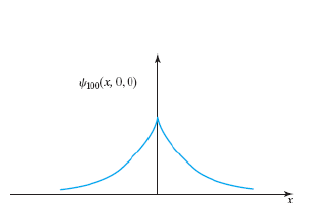
\includegraphics[width=0.4\textwidth]{Figures/6.7.png}
        \caption{氢原子基态波函数中的尖点}
        \label{fig:6.7}
    \end{figure}

    我们用三个下标来表示氢原子束缚态波函数,分别表示 $n$、$l$ 和 $m$ 的值。在另一种表示中,$l$ 的值用字母表示:
    \begin{equation}
        \begin{array}{|c|c|c|c|c|c|c|c|c|c|}
            \hline
            \text{字母} & s & p & d & f & g & h & i & k & \ldots \\
            \hline
            l & 0 & 1 & 2 & 3 & 4 & 5 & 6 & 7 & \ldots \\
            \hline
        \end{array}
        \label{eq:6.110}
    \end{equation}
    字母 $s$、$p$、$d$、$f$ 源于光谱学,分别代表尖锐(sharp)、主要(principal)、扩散(diffuse)和基本(fundamental)。之后,我们按字母顺序排列,只是省略了 $j$。在 $l$ 的字母前,我们写上 $n$ 的值。因此,基态波函数$\psi_{100}$ 可以写成 $\psi_{1s}$或更简单的$1s$。

\subsection*{$n=2$的波函数}

    对于$n=2$,我们有状态$\psi_{200}$、$\psi_{21-1}$、$\psi_{210}$、$\psi_{211}$。我们将$\psi_{200}$表示为$\psi_{2s}$或简单的$2s$。为了区分三个$2p$函数,我们使用下标来表示 $m$ 值,并将它们表示为$2p_1$、$2p_0$和$2p_{-1}$。从 (\ref{eq:6.100}) 可以看出,波函数中的径向因子取决于 $n$ 和 $l$,但不取决于 $m$。因此,三个 $2p$ 波函数都具有相同的径向因子。根据 (\ref{eq:6.100}) 和 (\ref{eq:6.99}) 可以用通常的方法求出 $2s$ 和 $2p$ 的径向因子,然后进行归一化处理。结果见表 \ref{tab:6.1}。请注意,$n=2$ 径向函数中的指数因子与 $R_{1s}$ 函数中的指数因子不同。将径向因子乘以适当的球谐函数,就能得到完整的波函数。使用(\ref{eq:6.101})、表\ref{tab:6.1}和表\ref{tab:5.1},我们有
    \begin{equation}
        2s = \frac{1}{2\pi^{1/2}}\left(\frac{Z}{a}\right)^{3/2}\left(1 - \frac{Zr}{2a}\right)\mathrm{e}^{-Zr/2a}
        \label{eq:6.111}
    \end{equation}
    \begin{equation}
        2p_{-1} = \frac{1}{8\pi^{1/2}}\left(\frac{Z}{a}\right)^{5/2}r\mathrm{e}^{-Zr/2a}\sin\theta\:\mathrm{e}^{-\mathrm{i}\phi}
        \label{eq:6.112}
    \end{equation}
    \begin{equation}
        2p_0 = \frac{1}{2\pi^{1/2}}\left(\frac{Z}{a}\right)^{5/2}r\mathrm{e}^{-Zr/2a}\cos\theta
        \label{eq:6.113}
    \end{equation}
    \begin{equation}
        2p_1 = \frac{1}{8\pi^{1/2}}\left(\frac{Z}{a}\right)^{5/2}r\mathrm{e}^{-Zr/2a}\sin\theta\:\mathrm{e}^{\mathrm{i}\phi}
        \label{eq:6.114}
    \end{equation}
    \begin{table}[htbp]
        \centering
        \caption{类氢原子波函数的径向因子}
        \label{tab:6.1}
        \renewcommand{\arraystretch}{1.5}
        \begin{tabular}{l}
            \hline
            $R_{1s} = 2\left(\frac{Z}{a}\right)^{3/2}\mathrm{e}^{-Zr/a}$ \\[0.5ex]
            \hline
            $R_{2s} = \frac{1}{\sqrt{2}}\left(\frac{Z}{a}\right)^{3/2}\left(1 - \frac{Zr}{2a}\right)\mathrm{e}^{-Zr/2a}$ \\[0.5ex]
            \hline
            $R_{2p} = \frac{1}{2\sqrt{6}}\left(\frac{Z}{a}\right)^{5/2}r\mathrm{e}^{-Zr/2a}$ \\[0.5ex]
            \hline
            $R_{3s} = \frac{2}{3\sqrt{3}}\left(\frac{Z}{a}\right)^{3/2}\left(1 - \frac{Zr}{3a} + \frac{2Z^2r^2}{27a^2}\right)\mathrm{e}^{-Zr/3a}$ \\[0.5ex]
            \hline
            $R_{3p} = \frac{8}{27\sqrt{6}}\left(\frac{Z}{a}\right)^{3/2}\left(\frac{Zr}{a} - \frac{Z^2r^2}{6a^2}\right)\mathrm{e}^{-Zr/3a}$ \\[0.5ex]
            \hline
            $R_{3d} = \frac{4}{81\sqrt{30}}\left(\frac{Z}{a}\right)^{7/2}r^2\mathrm{e}^{-Zr/3a}$ \\[0.5ex]
            \hline
        \end{tabular}
    \end{table}

    表 \ref{tab:6.1} 列出了类氢波函数中的一些归一化径向因子。图 \ref{fig:6.8} 是一些径向函数的示意图。除了$s$状态以外,因子$r^l$使得径向函数在$r=0$处为零。
    \begin{figure}[ht]
        \centering
        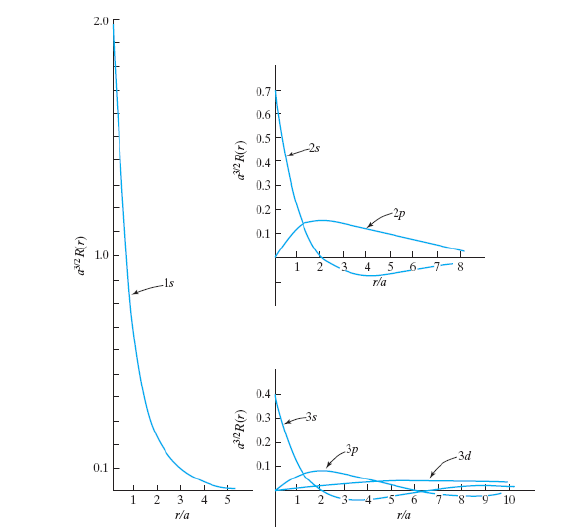
\includegraphics[width=0.9\textwidth]{Figures/6.8.png}
        \caption{
                \centering\parbox{\linewidth}{
                \centering
                氢原子($Z=1$)波函数\\
                径向因子$R_{nl}\left(r\right)$的示意图。\\
                所有图表都使用了相同的比例尺。\\
                (在某些课本中,这些函数没有按比例绘制)。
            }
        }
        \label{fig:6.8}
    \end{figure}

\subsection*{径向分布函数}

    在空间中位于$r$到$r+\mathrm{d}r$、$\theta$到$\theta+\mathrm{d}\theta$、$\phi$到$\phi+\mathrm{d}\phi$的体积微元内找到电子的概率为[式(\ref{eq:5.78})]
    \begin{equation}
        \left|\psi\right|^2\mathrm{d}\tau = \left[R_{nl}\left(r\right)\right]^2\left|Y_l^m\left(\theta,\phi\right)\right|^2r^2\sin\theta\:\mathrm{d}r\:\mathrm{d}\theta\:\mathrm{d}\phi
        \label{eq:6.115}
    \end{equation}
    我们现在想知道:在不限制 $\theta$ 和 $\phi$ 值的情况下,电子的径向坐标介于 $r$ 和 $r + \mathrm{d}r$ 之间的概率是多少?我们想知道在以原点为中心的薄球壳中找到电子的概率,其内半径为$r$,外半径为 $r + \mathrm{d}r$。因此,我们必须在保持 $r$ 不变的情况下,将 $\theta$ 和 $\phi$ 所有可能值的无穷小概率 (\ref{eq:6.115}) 相加。这相当于在 $theta$ 和 $\phi$ 上对 (\ref{eq:6.115}) 进行积分。因此,在$r$到$r+\mathrm{d}r$的区间内找到电子的概率为
    \begin{equation}
        \left[R_{nl}\left(r\right)\right]^2r^2\mathrm{d}r\int_{0}^{2\pi}\int_{0}^{\pi}\left|Y_l^m\left(\theta,\phi\right)\right|^2\sin\theta\:\mathrm{d}\theta\:\mathrm{d}\phi = \left[R_{nl}\left(r\right)\right]^2r^2\mathrm{d}r
        \label{eq:6.116}
    \end{equation}
    其中,我们用到了球谐函数是归一化的:
    \begin{equation}
        \boxed{
            \int_{0}^{2\pi}\int_{0}^{\pi}\left|Y_l^m\left(\theta,\phi\right)\right|^2\sin\theta\:\mathrm{d}\theta\:\mathrm{d}\phi = 1
        }
        \label{eq:6.117}
    \end{equation}
    从 (\ref{eq:5.72}) 和 (\ref{eq:5.80}) 可以看出。函数$R^2\left(r\right)r^2$决定了在距离原子核 $r$ 处找到电子的概率,称为\textbf{径向分布函数}(radial distribution function);见图 \ref{fig:6.9}。
    \begin{figure}[ht]
        \centering
        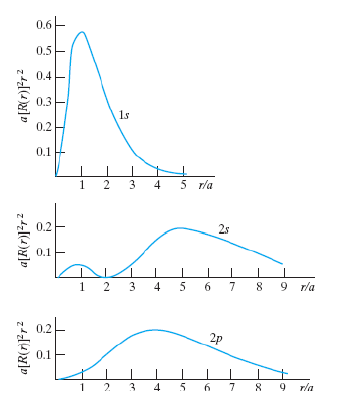
\includegraphics[width=0.5\textwidth]{Figures/6.9.png}
        \caption{氢原子径向分布函数$\left[R_{nl}\left(r\right)\right]^2r^2$的图象。}
        \label{fig:6.9}
    \end{figure}

    对于氢原子的$1s$基态,概率密度$\left|\psi\right|^2$由式(\ref{eq:6.104})给出,等于$\mathrm{e}^{-2r/a}$乘上一个常数,因此$\left|\psi_{1s}\right|^2$在$r=0$处达到最大值(见图\ref{fig:6.14})。然而,径向分布函数$\left[R_{1s}\left(r\right)\right]^2r^2$在原点处为零,而在$r=a$处达到最大值(见图 \ref{fig:6.9})。这两个事实并不矛盾。概率密度$\left|\psi\right|^2$与在体积为 $\mathrm{d}x\mathrm{d}y\mathrm{d}z$ 的无限小盒子中找到电子的概率成正比,而这一概率在原子核处为最大值。径向分布函数与在内外半径分别为 $r$ 和 $r +\mathrm{d}r$ 的薄球壳中找到电子的概率成正比,这一概率在$r = a$ 处达到最大值。由于$\psi_{1s}$只与$r$有关,$1s$ 的概率密度在薄球壳中基本恒定。如果我们把薄壳想象成无数个无穷小的盒子,每个盒子的体积都是 $\mathrm{d}x\mathrm{d}y\mathrm{d}z$,那么我们就可以把在薄壳中每个小盒子里的概率 $\left|\psi_{1s}\right|^2\mathrm{d}x\mathrm{d}y\mathrm{d}z$ 相加,得到在薄壳中找到电子的概率是$\left|\psi_{1s}\right|^2V_{\text{shell}}$。薄壳的体积 $V_{\text{shell}}$ 为
    \begin{equation*}
        \frac{4}{3}\pi\left(r+\mathrm{d}r\right)^3 - \frac{4}{3}\pi r^3 = 4\pi r^2\mathrm{d}r
    \end{equation*}
    其中$\left(\mathrm{d}r\right)^2$和$\left(\mathrm{d}r\right)^3$与$\mathrm{d}r$相比可以忽略。因此,位于薄壳中的概率是
    \begin{equation*}
        \left|\psi_{1s}\right|^2V_{\text{shell}} = R_{1s}^2\left(Y_0^0\right)^24\pi r^2\mathrm{d}r = R_{1s}^2\left[\left(4\pi\right)^{-1/2}\right]^24\pi r^2\mathrm{d}r = R_{1s}^2r^2\mathrm{d}r
    \end{equation*}
    与(\ref{eq:6.116})一致。$1s$ 径向分布函数在 $r =0$ 时为零,因为当 $r$ 变为零时,薄球壳的体积 $4\pi r^2\mathrm{d}r$ 变为零。它们的乘积$\left|\psi_{1s}\right|^24\pi r^2\mathrm{d}r$在$r=a$处达到最大值。

    \begin{examplebox}
        \textbf{例题:}求基态 \ce{H} 原子中电子与原子核的距离小于 $a$ 的概率。
        \\

        我们希望找到径向坐标介于$0$到$a$之间的概率。将处于 $r$ 和 $r +\mathrm{d}r$ 之间的无穷小概率 (\ref{eq:6.116}) 在 $0$ 到 $a$ 的范围内求和,就可以得出这个结果。这个无穷小量之和就是定积分
        \begin{equation*}
            \begin{aligned}
                \int_{0}^{a}R_{nl}^2r^2\mathrm{d}r & = \frac{4}{a^3}\int_{0}^{a}\mathrm{e}^{-2r/a}r^2\mathrm{d}r  = \left. -\frac{4}{a^3}\mathrm{e}^{-2r/a}\left(-\frac{r^a}{2} - \frac{2ra^2}{4} - \frac{2a^3}{8}\right)\right|_{0}^{a}\\
                & = 4\left[\mathrm{e}^{-2}\left(-5/4\right)- \left(-1/4\right)\right] = 0.323          
            \end{aligned}
        \end{equation*}
        其中$R_{10}$来自表\ref{tab:6.1},用到了附录中的积分A.7。
        \\

        \textbf{练习:}求 $2p_1$ \ce{H} 原子中电子与原子核的距离小于 $a$ 的概率。使用积分表或网站integrals.wolfram.com。(\textit{答案:}$0.00366$。)
    \end{examplebox}

\subsection*{实际类氢函数}

    除了$m=0$以外,因子$\mathrm{e}^{\mathrm{i}m\phi}$使得球谐函数为复数。化学家通常不使用 (\ref{eq:6.112}) 和 (\ref{eq:6.114}) 等复波函数,而是使用由复函数的线性组合形成的实类氢波函数。第 \ref{sec:3.6 Degeneracy} 节的定理给出了这一步骤的理由:简并能级的任何本征函数的线性组合都是具有相同本征值的哈密顿算符的本征函数。由于氢原子的能量与$m$无关,状态$2p_1$和$2p_{-1}$属于一个简并的能级。它们的任何线性组合都是哈密顿算符的本征函数,具有相同的能量本征值。

    将这两个函数组合起来得到一个实函数的方法是
    \begin{equation}
        2p_x \equiv \frac{1}{\sqrt{2}}\left(2p_1 + 2p_{-1}\right) = \frac{1}{4\sqrt{2\pi}}\left(\frac{Z}{a}\right)^{5/2}r\mathrm{e}^{-Zr/2a}\sin\theta\cos\phi
        \label{eq:6.118}
    \end{equation}
    其中,我们用到了(\ref{eq:6.112})、(\ref{eq:6.114})和$\mathrm{e}^{\pm \mathrm{i}\phi} = \cos\phi \pm \mathrm{i}\sin\phi$。因子$1/\sqrt{2}$使得波函数$2p_x$归一化:
    \begin{equation*}
        \begin{aligned}
            \int\left|2p_x\right|^2\mathrm{d}\tau & = \frac{1}{2}\left(\int\left|2p_1\right|^2\mathrm{d}\tau + \int\left|2p_{-1}\right|^2\mathrm{d}\tau + \int\left(2p_{-1}\right)^{\ast}2p_1\mathrm{d}\tau + \int\left(2p_{1}\right)^{\ast}2p_{-1}\mathrm{d}\tau\right)\\
            & = \frac{1}{2}\left(1 + 1 + 0 + 0\right) = 1
        \end{aligned}
    \end{equation*}
    其中我们用到了$2p_1$和$2p_{-1}$是归一化且互相正交的性质,因为
    \begin{equation*}
        \int_{0}^{2\pi}\left(\mathrm{e}^{\mathrm{i}\phi}\right)^{\ast}\mathrm{e}^{\mathrm{i}\phi}\mathrm{d}\phi = \int_{0}^{2\pi}\mathrm{e}^{2\mathrm{i}\phi}\mathrm{d}\phi = 0
    \end{equation*}
    如果我们注意到 (\ref{eq:5.51}) 给出了 下式,那么 (\ref{eq:6.118}) 的命名$2p_x$就会更加清晰:
    \begin{equation}
        2p_x = \frac{1}{4\sqrt{2\pi}}\left(\frac{Z}{a}\right)^{5/2}x\mathrm{e}^{-Zr/2a}
        \label{eq:6.119}
    \end{equation}

    第二种组合函数的方法是
    \begin{equation}
        2p_y \equiv \frac{1}{\mathrm{i}\sqrt{2}}\left(2p_1 - 2p_{-1}\right) = \frac{1}{4\sqrt{2\pi}}\left(\frac{Z}{a}\right)^{5/2}r\sin\theta\sin\phi\:\mathrm{e}^{-Zr/2a}
        \label{eq:6.120}
    \end{equation}
    \begin{equation}
        2p_y = \frac{1}{4\sqrt{2\pi}}\left(\frac{Z}{a}\right)^{5/2}y\mathrm{e}^{-Zr/2a}
        \label{eq:6.121}
    \end{equation}
    函数$2p_0$是实数,通常用下式表示:
    \begin{equation}
        2p_0 = 2p_z = \frac{1}{\sqrt{\pi}}\left(\frac{Z}{a}\right)^{5/2}z\mathrm{e}^{-Zr/2a}
        \label{eq:6.122}
    \end{equation}
    其中大写的$Z$表示核中的质子数,小写的$z$为电子的$z$坐标。函数$2p_x$、$2p_y$和$2p_z$是互相正交的。注意$2p_z$在$xOy$平面内为零,在该平面上方为正,在下方为负。

    函数$2p_{-1}$和$2p_1$都是算符$\hat{L}^2$的本征函数,其本征值也相同,为$2\hbar^2$。第 3.6 节的推理表明,线性组合 (\ref{eq:6.118}) 和 (\ref{eq:6.120}) 也是 $\hat{L}^2$ 的本征函数,其本征值为 $2\hbar^2$ 。然而,$2p_{-1}$和$2p_1$是$\hat{L}_z$的本征函数,但本征值分别为$-\hbar$和$\hbar$。因此,$2p_x$和$2p_y$不是$\hat{L}_z$的本征函数。

    我们可以推广这一过程,为更高的状态构建实波函数。由于 $m$ 的范围是从 $- l$ 到 $+ l$,对于每个包含因子$\mathrm{e}^{-\mathrm{i}\left|m\right|\phi}$的复函数,都有一个 $n$ 和 $l$ 值相同但包含因子$\mathrm{e}^{+\mathrm{i}\left|m\right|\phi}$的函数,将这些函数相减,得到两个实函数,其中一个具有因子$\cos\left(\left|m\right|\phi\right)$,另一个具有因子$\sin\left(\left|m\right|\phi\right)$。表 \ref{tab:6.2} 列出了类氢原子的实波函数。这些函数的下标来自与 $2p_x$ 、$2p_y$ 和 $2p_z$ 函数类似的考虑。例如,$3d_{x}$ 函数与 $xy$ 成正比(问题 6.37)。

    实类氢波函数由复函数导出,方法如下:当$m \neq 0$时,将$\mathrm{e}^{\mathrm{i}m\phi}/\left(2\pi\right)^{1/2}$替换为$\pi^{-1/2}\cos\left(\left|m\right|\phi\right)$或$\pi^{-1/2}\sin\left(\left|m\right|\phi\right)$;当$m=0$时,对于实函数和复函数,$\phi$因子都为$1/\left(2\pi\right)^{1/2}$。

    在处理分子时,实类氢轨道比复类氢轨道更有用。例如,我们将在第 节中看到,氧原子的实原子轨道 $2p_x$、$2p_y$ 和 $2p_z$具有适当的对称性,可用于构建 \ce{H2O} 分子的波函数,而复数 $2p$ 轨道则不具备这种对称性。

    \begin{table}[htbp]
        \centering
        \caption{类氢原子的实波函数}
        \label{tab:6.2}
        \renewcommand{\arraystretch}{1.5}
        \begin{tabular}{l}
            \hline
            $1s = \frac{1}{\pi^{1/2}}\left(\frac{Z}{a}\right)^{3/2}e^{-Zr/a}$ \\[0.5ex]
            \hline
            $2s = \frac{1}{4\left(2\pi\right)^{1/2}}\left(\frac{Z}{a}\right)^{3/2}\left(2 - \frac{Zr}{2a}\right)e^{-Zr/2a}$ \\[0.5ex]
            \hline
            $2p_z = \frac{1}{4\left(2\pi\right)^{1/2}}\left(\frac{Z}{a}\right)^{5/2}r\mathrm{e}^{-Zr/2a}\cos\theta$ \\[0.5ex]
            \hline
            $2p_x = \frac{1}{4\left(2\pi\right)^{1/2}}\left(\frac{Z}{a}\right)^{5/2}r\mathrm{e}^{-Zr/2a}\sin\theta\:\cos\phi$ \\[0.5ex]
            \hline
            $2p_y = \frac{1}{4\left(2\pi\right)^{1/2}}\left(\frac{Z}{a}\right)^{5/2}r\mathrm{e}^{-Zr/2a}\sin\theta\:\sin\phi$ \\[0.5ex]
            \hline
            $3s = \frac{1}{81\left(3\pi\right)^{1/2}}\left(\frac{Z}{a}\right)^{3/2}\left(27 - 18\frac{Zr}{a} + 2\frac{Z^2r^2}{a^2}\right)e^{-Zr/3a}$ \\[0.5ex]
            \hline
            $3p_z = \frac{2^{1/2}}{81\pi^{1/2}}\left(\frac{Z}{a}\right)^{5/2}\left(6 - \frac{Zr}{a}\right)r\mathrm{e}^{-Zr/3a}\cos\theta$ \\[0.5ex]
            \hline
            $3p_x = \frac{2^{1/2}}{81\pi^{1/2}}\left(\frac{Z}{a}\right)^{5/2}\left(6 - \frac{Zr}{a}\right)r\mathrm{e}^{-Zr/3a}\sin\theta\:\cos\phi$ \\[0.5ex]
            \hline
            $3p_y = \frac{2^{1/2}}{81\pi^{1/2}}\left(\frac{Z}{a}\right)^{5/2}\left(6 - \frac{Zr}{a}\right)r\mathrm{e}^{-Zr/3a}\sin\theta\:\sin\phi$ \\[0.5ex]
            \hline
            $3d_{z^2} = \frac{1}{81\left(6\pi\right)^{1/2}}\left(\frac{Z}{a}\right)^{7/2}r^2\mathrm{e}^{-Zr/3a}\left(3\cos^2\theta - 1\right)$ \\[0.5ex]
            \hline
            $3d_{xz} = \frac{2^{1/2}}{81\left(6\pi\right)^{1/2}}\left(\frac{Z}{a}\right)^{7/2}r^2\mathrm{e}^{-Zr/3a}\sin\theta\:\cos\theta\:\cos\phi$ \\[0.5ex]
            \hline
            $3d_{yz} = \frac{2^{1/2}}{81\left(6\pi\right)^{1/2}}\left(\frac{Z}{a}\right)^{7/2}r^2\mathrm{e}^{-Zr/3a}\sin\theta\:\cos\theta\:\sin\phi$ \\[0.5ex]
            \hline
            $3d_{x^2-y^2} = \frac{1}{81\left(2\pi\right)^{1/2}}\left(\frac{Z}{a}\right)^{7/2}r^2\mathrm{e}^{-Zr/3a}\sin^2\theta\:\cos2\phi$ \\[0.5ex]
            \hline
            $3d_{xy} = \frac{1}{81\left(2\pi\right)^{1/2}}\left(\frac{Z}{a}\right)^{7/2}r^2\mathrm{e}^{-Zr/3a}\sin^2\theta\:\sin2\phi$ \\[0.5ex]
        \end{tabular}
    \end{table}

\section{类氢轨道}
\label{sec:6.7 Hydrogenlike orbitals}
    类氢波函数是单电子空间波函数,类氢轨道也是单电子空间波函数(第 \ref{sec:6.5 The Hydrogen Atom} 节)。这些函数是针对单电子原子得出的,我们不能指望用它们来真正准确地表示多电子原子的波函数。第 \ref{chap:11} 章将讨论如何使用轨道概念来近似多电子原子的波函数。现在我们只讨论单电子原子。

    描绘轨道有两种完全不同的方法。一种方法是绘制函数图象;第二种方法是绘制概率密度恒定的等值面。

    首先考虑绘制函数图象。要将 $\psi$ 的变化绘制成三个自变量 $r$、$\theta$ 和 $\phi$ 的函数,我们需要四个维度。我们世界的三维特性使我们无法绘制这样的图表。因此,我们绘制$\psi$中某个因子的图象。绘制$R\left(r\right)$与$r$的关系图,我们得到图 \ref{fig:6.8} 的曲线,其中不包含 $\psi$ 角度变化的任何信息。
    \begin{figure}[ht]
        \centering
        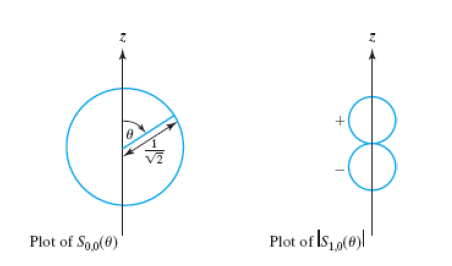
\includegraphics[width=0.5\textwidth]{Figures/6.10.png}
        \caption{氢原子波函数中 $s$ 和 $p_z$ 的 $\theta$ 因子的极坐标图。}
        \label{fig:6.10}
    \end{figure}

    现在来考虑$S\left(\theta\right)$的图象,由表(\ref{tab:5.1}),我们有
    \begin{equation*}
        S_{0,0} = 1/\sqrt{2}, \quad S_{1,0} = \frac{1}{2}\sqrt{6}\cos\theta
    \end{equation*}
    我们可以使用二维直角坐标绘制这些函数的图象,在纵轴上绘制 $S$,在横轴上绘制 $\theta$。$S_{0,0}$给出了一条水平直线,而$S_{1,0}$给出了一条余弦曲线。更常见的情况是使用平面极坐标系绘制$S$的图象。变量$\theta$是与$z$轴正半轴的夹角,而$S\left(\theta\right)$是从原点到图上点的距离。对于$S_{0,0}$我们得到了一个圆;对于$S_{1,0}$,我们得到了两个相切的圆(图\ref{fig:6.10})。$S_{1,0}$图像中较低的圆旁边的负号,表示当$\frac{1}{2}\pi < \theta \leq \pi$时,$S_{1,0}$为负值。严格来说,在绘制 $\cos\theta$ 时,我们只得到了较高的圆,它被绘制了两次;要得到两个相切的圆,我们必须绘制 $\left|\cos\theta\right|$ 。

    我们可以绘制一张$\left|S\left(\theta\right)T\left(\phi\right)\right|$与$\theta$和$\phi$的函数关系图,而不是分别绘制角向因子的图象。我们将使用球坐标,从原点到图上点的距离将为$\left|S\left(\theta\right)T\left(\phi\right)\right|$。对于$s$状态,$ST$与角度无关,因此我们得到了一个半径为$1/\left(4\pi\right)^{1/2}$的球面。而对于$p_z$状态,$ST = \frac{1}{2}\left(3/\pi\right)^{1/2}\cos\theta$,$\left|ST\right|$的图象由两个球体组成,球体中心位于 $z$ 轴,并与原点相切(图 \ref{fig:6.11})。毫无疑问,图 \ref{fig:6.11} 是大家都很熟悉的。有些书上说这给出了 $p_z$ 轨道的形状,这是错误的。图 \ref{fig:6.11} \textit{只是一张波函数 $p_z$ 中的角向因子图。}角向因子 $p_x$ 和 $p_y$ 的图形分别给出了位于 $x$ 和 $y$ 轴上的切线球。如果我们以球面坐标绘制 $S^2T^2$,就会得到具有我们熟悉的八字形截面的表面;重复一遍,这些是图形,而不是轨道形状。
    \begin{figure}[ht]
        \centering
        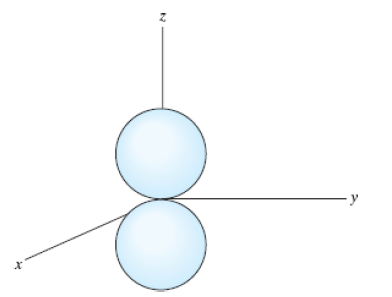
\includegraphics[width=0.4\textwidth]{Figures/6.11.png}
        \caption{
            $p_z$波函数中角向因子$\left|Y_1^0\left(\theta,\phi\right)\right|$的图象。
        }
        \label{fig:6.11}
    \end{figure}

    现在,考虑绘制概率密度恒定的等值面。我们将在空间中画出曲面,在每个曲面上,概率密度 $\left|\psi\right|^2$ 的值都是恒定的。自然,如果 $\left|\psi\right|^2$ 在给定的曲面上是常数,那么 $\left|\psi\right|$ 在该曲面上也是常数。$\left|\psi\right|^2$ 和 $\left|\psi\right|$ 的等值面是相同的。

    对于$s$轨道,$\psi$只与$r$有关,等值面就是一个恒定 $r$ 的曲面,即以原点为中心的球面。为了确定一个轨道的大小,我们取一个等值面,在这个等值面内找到电子的概率比如说是 $95\%$,因此我们希望$\int_{V}\left|\psi\right|^2\mathrm{d}\tau = 0.95$,其中$V$是轨道等值面所包围的体积。

    让我们来计算类氢轨道 $2p_y$ 在 $yOz$ 平面上的横截面。在该平面上,有$\phi = \pi/2$(图\ref{fig:6.5})以及$\sin\phi = 1$;因此表 \ref{tab:6.2} 给出了该轨道在 $yOz$ 平面上的情况
    \begin{equation}
        \left|2p_y\right| = k^{5/2}\pi^{-1/2}r\mathrm{e}^{-kr}\left|\sin\theta\right|
        \label{eq:6.123}
    \end{equation}
    其中$k = Z/2a$。为了找到轨道横截面,我们使用平面极坐标来绘制 $\psi$ 固定值的 (\ref{eq:6.123}) 图;$r$是到原点的距离,而$\theta$是与 $z$ 轴的夹角。图 \ref{fig:6.12} 显示了典型等值线的结果(问题 6.44)。由于$y\mathrm{e}^{-kr} = y\exp\left[-k\left(x^2+y^2+z^2\right)^{1/2}\right]$,我们可以看到$2p_y$轨道是$y$和$\left(x^2+z^2\right)$的函数。因此,在以 $y$ 轴为中心、平行于 $xOz$ 平面的圆上,$2p_y$是常数。因此,将图 \ref{fig:6.12} 中的横截面绕 $y$ 轴旋转,可以得到一对扭曲的椭圆体,从而形成三维等值面。实际 $2p$ 轨道的形状是两个分离的扭曲椭圆体,而不是两个相切的球体。
    \begin{figure}[ht]
        \centering
        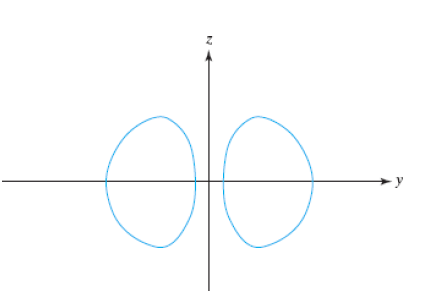
\includegraphics[width=0.45\textwidth]{Figures/6.12.png}
        \caption{$2p_y$轨道等值线。}
        \label{fig:6.12}
    \end{figure}

    现在来考虑两个复轨道$2p_{\pm 1}$的形状。我们有
    \begin{equation*}
        2p_{\pm 1} = k^{5/2}\pi^{-1/2}r\mathrm{e}^{-kr}\sin\theta\:\mathrm{e}^{\pm \mathrm{i}\phi}
    \end{equation*}
    \begin{equation}
        \left|2p_{\pm 1}\right| = k^{5/2}\pi^{-1/2}\mathrm{e}^{-kr}r\left|\sin\theta\right|
        \label{eq:6.124}
    \end{equation}
    这两个轨道有相同的形状。由于 (\ref{eq:6.124}) 和 (\ref{eq:6.123}) 的右边相同,我们得出结论:图 \ref{fig:6.12} 也给出了 $yOz$ 平面上 $2p_{\pm 1}$ 轨道的横截面。由于[式(\ref{eq:5.51})]
    \begin{equation*}
        \mathrm{e}^{-kr}r\left|\sin\theta\right| = \exp\left[-k\left(x^2+y^2+z^2\right)^{1/2}\right]\left(x^2+y^2\right)^{1/2}
    \end{equation*}
    我们看到$2p_{\pm 1}$轨道是$z$和$\left(x^2+y^2\right)$的函数,因此,我们将图 \ref{fig:6.12} 绕 $z$ 轴旋转,就能得到三维轨道形状。这样就形成了一个甜甜圈状的表面。

    图 6.13 显示了一些类氢轨道面。$2s$ 轨道有一个看不到的球形节点;$3s$ 轨道有两个这样的节点。$3p_z$ 轨道有一个球形节点(虚线表示)和一个节点平面($xOy$ 平面)。$3d_{z^2}$ 轨道有两个节点锥。$3d_{x^2-y^2}$ 轨道有两个节平面。请注意,不同轨道的视图并不相同。波函数的相对符号已标出。表 \ref{tab:6.2} 中的其他三个实 $3d$ 轨道与 $3d_{x^2-y^2}$ 轨道形状相同,但方向不同。$3d_{xy}$轨道的裂片位于$x$轴和$y$轴之间,它是通过将$3d_{x^2-y^2}$轨道绕$z$轴旋转\ang{45}而得到的。$3d_{yz}$ 和 $3d_{xz}$ 轨道的裂片分别位于 $y$ 轴和 $z$ 轴之间以及 $x$ 轴和 $z$ 轴之间。(真实类氢轨道的在线三维视图见 \url{www.falstad.com/qmatom};可使用鼠标旋转)
    \begin{figure}[ht]
        \centering
        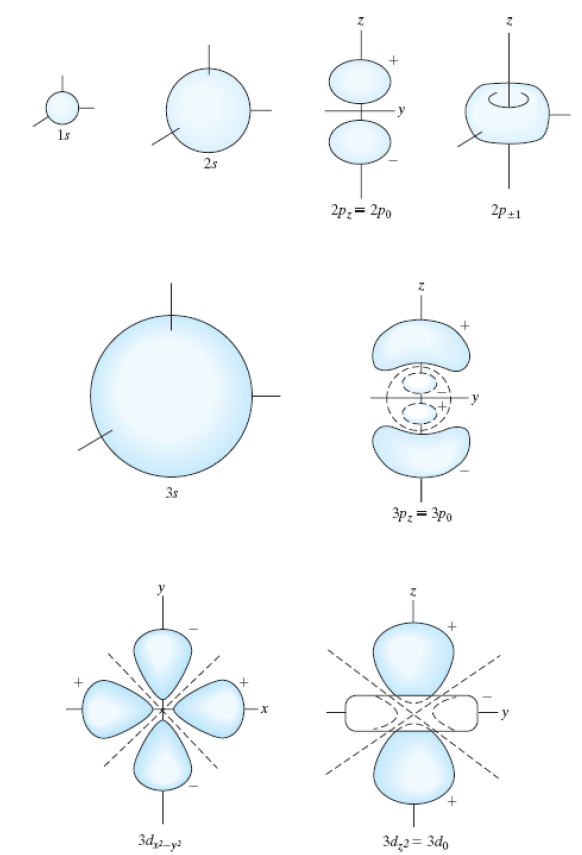
\includegraphics[width=0.65\textwidth]{Figures/6.13.png}
        \caption{一些氢原子轨道的形状。}
        \label{fig:6.13}
    \end{figure}
    \begin{figure}[ht]
        \centering
        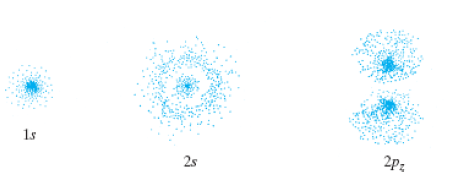
\includegraphics[width=0.6\textwidth]{Figures/6.14.png}
        \caption{
                \centering\parbox{\linewidth}{
                \centering
                一些氢原子状态的概率密度。\\
                有关精确的立体图,请参见D. T. Cromer, \textit{J. Chem. Educ.}, \textbf{45}, 626 (1968).
            }
        }
        \label{fig:6.14}
    \end{figure}

    图 \ref{fig:6.14} 表示各种轨道在 $yOz$ 平面上的概率密度。特定区域中点的数量与该区域中的 $\left|\psi\right|^2$ 值成正比。将这些图表绕垂直($z$)轴旋转,就得到了三维概率密度。$2s$ 轨道的角度系数是一个常数,因此没有角向节点;对于这个轨道,$n-l-1=1$,表明有一个径向节点。图 \ref{fig:6.14} 显示了 $\psi_{2s}=0$ 的球面。

    薛定谔最初对$\left|\psi\right|^2$的解释是,电子被 “涂抹 ”成电子云。如果我们考虑一个电子从一种介质传递到另一种介质,我们会发现 $\left|\psi\right|^2$ 在两种介质中都不为零。根据电子云的解释,这意味着电子的一部分被反射,一部分被透射。然而,在实验中,我们永远无法检测到电子的一小部分;电子是不可分割的实体。根据玻恩解释,两种介质中的 $\left|\psi\right|^2$ 值给出了反射和透射的\textit{概率},从而解决了这一难题。我们绘制的轨道形状给出了找到电子的总概率为 $95\%$ 的空间区域。

\section{塞曼效应}
\label{sec:6.8 Zeeman effect}
    1896 年,塞曼(Zeeman)观察到外加磁场会导致原子光谱线分裂。我们将研究氢原子的\textit{塞曼效应}(Zeeman Effect)。我们首先回顾一下磁学。

    磁场产生于移动的电荷。速度为 $\mathbf{v}$ 的电荷 $Q$ 在空间 $P$ 点产生磁场 $\mathbf{B}$,其中
    \begin{equation}
        \mathbf{B} = \frac{\mu_0}{4\pi}\frac{Q\mathbf{v}\times\mathbf{r}}{r^3}
        \label{eq:6.125}
    \end{equation}
    其中$\mathbf{r}$是从电荷$Q$到点 $P$ 的位置矢量,$\mu_0$ [称为\textbf{真空磁导率}(permeability of vacuum)或\textbf{磁常数}(magnetic constant)]定义为$4\pi\times 10^{-7}\:\mathrm{N} \:\mathrm{C}^{-2}\: \mathrm{s}^{2}$。[公式 (\ref{eq:6.125}) 只适用于速度远小于光速的非加速电荷。]矢量$\mathbf{B}$称为\textbf{磁感应强度}(magnetic induction)或\textbf{磁通量}(magnetic flux density)。(以前认为矢量 $\mathbf{H}$ 是基磁场矢量,所以称 $\mathbf{H}$ 为\textit{磁场强度}。现在人们知道 $\mathbf{B}$ 是基磁场矢量)公式 (\ref{eq:6.125}) 采用国际单位制,$Q$ 单位为库仑,$\mathbf{B}$ 单位为特斯拉(Tesla) (T),其中$1\:\mathrm{T} = 1\:\mathrm{N}\:\mathrm{C}^{-1}\:\mathrm{m}^{-1} \: \mathrm{s}$。

    两个电荷 $+Q$ 和 $-Q$ 相隔很小的距离 $b$ 就构成了一个电偶极子。\textbf{电偶极矩}(electric dipole moment)被定义为从 $-Q$ 到 $+Q$ 的矢量,大小为 $Qb$。对于一个小的平面电流环,电流中的移动电荷所产生的磁场与电偶极子所产生的电场的数学表达式相同,只是电偶极矩被\textbf{磁偶极矩}(magnetic dipole moment) $\mathbf{m}$ 所取代;$\mathbf{m}$ 是一个大小为 $IA$ 的矢量,其中 $I$ 是在面积为 $A$ 的环中流动的电流。$\mathbf{m}$ 的方向与电流回路的平面垂直。

    考虑与以速度 $v$ 在半径为 $r$ 的圆内运动的电荷 $Q$ 有关的磁(偶极)子。电流是单位时间内的电荷流量。圆的周长为$2\pi r$,旋转一周的时间为$2\pi r/v$。因此,电流为$I = Qv/2\pi r$。因此,磁偶极矩$\mathbf{m}$的大小为
    \begin{equation}
        \left|\mathbf{m}\right| = IA = \left(Qv/2\pi r\right)\pi r^2 = Qvr/2 = Qrp/2m
        \label{eq:6.126}
    \end{equation}
    其中$m$是带电粒子的质量,$p$为其动量。由于径向矢量$\mathbf{r}$与$\mathbf{p}$垂直,我们有
    \begin{equation}
        \mathbf{m}_L = \frac{Q\mathbf{r}\times\mathbf{p}}{2m} = \frac{Q}{2m}\mathbf{L}
        \label{eq:6.127}
    \end{equation}
    其中我们用到了轨道角动量$\mathbf{L}$的定义,$\mathbf{m}$的下标表示它来源于粒子的轨道运动。虽然我们用圆周运动的特殊情况得出了 (\ref{eq:6.127}),但其有效性是普遍的。对于一个电子,$Q = -\mathrm{e}$,因其轨道运动而产生的磁矩为
    \begin{equation}
        \mathbf{m}_L = -\frac{\mathrm{e}}{2m_{\mathrm{e}}}\mathbf{L}
        \label{eq:6.128}
    \end{equation}
    矢量$\mathbf{L}$的大小由(\ref{eq:5.95})给出,而具有轨道角动量子数 $l$ 的电子的轨道磁矩大小为
    \begin{equation}
        \left|\mathbf{m}_L\right| = \frac{\mathrm{e}\hbar}{2m_{\mathrm{e}}}\left[l\left(l+1\right)\right]^{1/2} = \mu_{B}\left[l\left(l+1\right)\right]^{1/2}
        \label{eq:6.129}
    \end{equation}
    常量$\mathrm{e}\hbar/2m_{\mathrm{e}}$称为\textit{玻尔磁子}(Bohr magneton),记作$\mu_{B}$:
    \begin{equation}
        \mu_{B} \equiv \mathrm{e}\hbar/2m_{\mathrm{e}} = 9.2740 \times 10^{-24}\: \mathrm{J}/\mathrm{T}
        \label{eq:6.130}
    \end{equation}

    现在我们来考虑给氢原子施加外部磁场。磁偶极子 $\mathbf{m}$ 与外部磁场 $\mathbf{B}$ 之间的相互作用能量可表示为
    \begin{equation}
        E_B = -\mathbf{m}\cdot\mathbf{B}
        \label{eq:6.131}
    \end{equation}
    使用式(\ref{eq:6.128}),我们有
    \begin{equation}
        E_{B} = \frac{\mathrm{e}}{2m_{\mathrm{e}}}\mathbf{L}\cdot\mathbf{B}
        \label{eq:6.132}
    \end{equation}
    我们沿外加磁场的方向确定$z$轴的位置:$\mathbf{B} = B\mathbf{k}$,其中$\mathbf{k}$是$z$方向的单位矢量。我们有
    \begin{equation*}
        E_B = \frac{\mathrm{e}}{2m_{\mathrm{e}}}B\left(L_x\mathbf{i} + L_y\mathbf{j} + L_z\mathbf{k}\right)\cdot\mathbf{k} = \frac{\mathrm{e}}{2m_{\mathrm{e}}}BL_z = \frac{\mu_B}{\hbar}BL_z
    \end{equation*}
    其中$L_z$是轨道角动量在$z$方向上的分量。我们现在将$L_z$替换为算符$\hat{L}_z$,在哈密顿算符中得到以下由外部磁场产生的附加项:
    \begin{equation}
        \hat{H}_B = \mu_BB\hbar^{-1}\hat{L}_z
        \label{eq:6.133}
    \end{equation}

    外加磁场中氢原子的薛定谔方程为
    \begin{equation}
        \left(\hat{H}+\hat{H}_B\right)\psi = E\psi
        \label{eq:6.134}
    \end{equation}
    其中,$\hat{H}$是在无外场作用下氢原子的哈密顿算符。我们很容易验证公式 (\ref{eq:6.134}) 的解就是复类氢波函数 (\ref{eq:6.61}) :
    \begin{equation}
        \left(\hat{H}+\hat{H}_B\right)R\left(r\right)Y_l^m\left(\theta,\phi\right) = \hat{H}RY_l^m + \mu_B\hbar^{-1}B\hat{L}_zRY_l^m = \left(-\frac{Z^2}{n^2}\frac{\mathrm{e}^2}{8\pi\varepsilon_0a}+\mu_BBm\right)RY_l^m
        \label{eq:6.135}
    \end{equation}
    其中用到了式(\ref{eq:6.94})和(\ref{eq:5.105})。因此,能量中存在一个附加项,而外部磁场消除了 $m$ 简并。由于显而易见的原因,$m$ 通常被称为\textit{磁量子数}(magnetic quantum number)。实际上,由于电子自旋磁矩的存在,观测到的能量偏移与公式 (\ref{eq:6.135}) 的预测值并不一致(第 \ref{chap:10} 章和第 \ref{sec:11.7 The Atomic Hamiltonian} 节。)

    在第 \ref{chap:5} 章中,我们发现在量子力学中,$\mathbf{L}$ 位于一个圆锥面上。对 $\mathbf{L}$ 在外加磁场中运动的\textit{经典}力学处理表明:场对 $\mathbf{m}_L$ 产生力矩,使 $\mathbf{L}$ 以 $\left|\mathbf{m}_L\right|B/2\pi \left|L\right|$ 给定的恒定频率绕 $\mathbf{B}$ 的方向旋转,同时与 $\mathbf{B}$ 保持恒定角度。这种脱落运动称为\textit{进动}(precession)。在量子力学中,完整指定$\mathbf{L}$是不可能的。然而,我们会发现$\left\langle \mathbf{L} \right\rangle$绕着场的方向进动。(\textit{Dicke and Wittke}, Section 12-3)

\section{径向薛定谔方程的数值解法}
\label{sec:6.9 Numerical Solution of the Radial Schrödinger Equation}
    对于单粒子中心力问题,波函数$\psi = R\left(r\right)Y_l^m\left(\theta,\phi\right)$由(\ref{eq:6.16})给出,径向因子$R\left(r\right)$通过求解径向方程(\ref{eq:6.17})得到。第\ref{sec:4.4 Numerical Solutions of the One-Dimensional Time-Independent Schrödinger Equation}节中的Numerov方法适用于形式为$\psi^{\prime\prime} = G\left(x\right)\psi\left(x\right)$的微分方程[式(\ref{eq:4.66})],为了应用该方法,我们需要消去(\ref{eq:6.17})中的一阶导数$R^{\prime}$。让我们定义$F\left(r\right) \equiv rR\left(r\right)$,则
    \begin{equation}
        R\left(r\right) = r^{-1}F\left(r\right)
        \label{eq:6.136}
    \end{equation}
    因此,$R^{\prime} = -r^{-2}F + r^{-1}F^{\prime}$,$R^{\prime\prime} = -2r^{-3}F + 3r^{-2}F^{\prime} - r^{-1}F^{\prime\prime}$。将这些表达式代入(\ref{eq:6.17}),将径向方程变换为
    \begin{equation}
        -\frac{\hbar^2}{2m}F^{\prime\prime}\left(r\right)+\left[V\left(r\right)+\frac{l\left(l+1\right)\hbar^2}{2mr^2}\right]F\left(r\right) = EF\left(r\right)
        \label{eq:6.137}
    \end{equation}
    \begin{equation}
        F^{\prime\prime}\left(r\right) = G\left(r\right)F\left(r\right), \quad \text{其中}G\left(r\right) \equiv \frac{m}{\hbar^2}\left(2V-2E\right)+ \frac{l\left(l+1\right)}{r^2}
        \label{eq:6.138}
    \end{equation}
    其形式符合了Numerov方法的要求。为了使用数值法解(\ref{eq:6.137}),我们需要分别处理每个$l$的值。方程 (\ref{eq:6.137}) 类似于一维薛定谔方程——$\left(\hbar^2/2m\right)\psi^{\prime\prime}\left(x\right)+V\left(x\right)\psi\left(x\right) = E\psi\left(x\right)$,只不过用$r$(范围是$0 \to \infty$)代替了$x$(范围是$-\infty$到$+\infty$),$F\left(r\right) \equiv rR\left(r\right)$代替了$\psi$,$V\left(r\right) + l\left(l+1\right)\hbar^2/2mr^2$代替了$V\left(x\right)$。我们可以预期,对于每个 $l$ 值,能量最低的解将有 $0$ 个内部节点(即$0<r<\infty$的节点),下一个最低的解将有 $1$ 个内部节点,依此类推。

    回顾式(\ref{eq:6.81})之后的讨论,若$R\left(r\right)$在原点附近表现与$1/r^b$相似,那么如果$b>1$,则$R\left(r\right)$不是平方可积的;值$b=1$是不允许的,如(\ref{eq:6.83})之后所述。因此,当$r=0$时,必须有$F\left(r\right)\equiv rR\left(r\right)$为零。

    对于$l\neq 0$的情况,(\ref{eq:6.138})中的$G\left(r\right)$在$r=0$处发散,这会让大多数电脑感到不爽。为了避免这个问题,我们可以从极小的$r$值开始求解(例如,$10^{-15}$为无量纲的$r_r$)并近似$F\left(r\right)$在该点为零。

    例如,我们将使用 Numerov 方法求解最低束缚态 \ce{H} 原子能量。有$V = -\mathrm{e}^2/4\pi\varepsilon_0r = -\mathrm{e}^{\prime^2}/r$,其中$\mathrm{e}^{\prime} \equiv \mathrm{e}/\left(4\pi\varepsilon_0\hbar^2/m\right)^{1/2}$。径向方程(\ref{eq:6.62})包含三个常数$\mathrm{e}^{\prime}$、$\mu$和$\hbar$,其中$\mathrm{e}^{\prime} \equiv \mathrm{e}/\left(4\pi\varepsilon_0\hbar^2/m\right)^{1/2}$具有国际单位$\mathrm{m}\: \mathrm{N}^{1/2}$(见附录的表A.1),因此,有无量纲的$\left[\mathrm{e}^{\prime}\right] = \mathrm{L}^{3/2}\mathrm{M}^{1/2}\mathrm{T}^{-1}$。按照公式(\ref{eq:4.73})的推导过程,我们发现 \ce{H} 原子的约化能量和约化径向坐标为(问题 6.47)
    \begin{equation}
        E_r = E/\mu \mathrm{e}^{\prime ^4}\hbar^{-2}, \quad r_r = r/B = r/\hbar^2\mu^{-1}\mathrm{e}^{\prime ^{-2}}
        \label{eq:6.139}
    \end{equation}
    使用(\ref{eq:6.139})、(\ref{eq:4.76})和(\ref{eq:4.77})将$\psi$替换为$F$,使用$B = \hbar^2\mu^{-1}\mathrm{e}^{\prime ^{-2}}$将氢原子的式(\ref{eq:6.137})变换为(问题6.47)
    \begin{equation}
        F^{\prime\prime}_r = G_rF_r, \quad \text{其中}G_r = l\left(l+1\right)/r_r^2 - 2/r_r -2E_r
        \label{eq:6.140}
    \end{equation}
    其中$F_r = F/B^{-1/2}$。

    氢原子束缚态能量均小于零。假设我们想知道$E_r \leq -0.04$的氢原子束缚态本征值。令该能量等于$V_r$,我们有(问题6.47)$-0.04 = -1/r_r$,而这个能量值的经典允许区域从$r_r = 0$一直延申到$r_r = 25$。进入经典禁区2个单位长度,我们有$r_{r,\max} = 27$并要求$F_r\left(27\right)=0$。我们将$s_r$设为0.1,将0到27均分为270个点(更准确地说,是$10^{-15}$到$27+10^{-15}$)。

    (\ref{eq:6.140})中的$G_r$包含参数$l$,所以必须修改表 4.1 中的程序,以输入 $l$ 的值。设置电子表格时,请在某个单元格中输入 $l$ 值,并在输入定义 $G_r$ 的单元格 B7 的公式时参考该单元格(图 4.9 4.8)。A列的起始位置为$r_r = 1\times 10^{-15}$。电子表格的 C 列将包含 $F_r$ 值,而不是 $\psi_r$ 值,$F_r$ 在 $r_r = 1\times10^{-15}$ 处与零相差很小,可以忽略不计,因此在该点将取为零。

    根据上述选择,我们可以找到(问题 6.48a )的最低三个$l=0$的 \ce{H} 原子本征值为$E_r = -4970,-0.1246,-0205499$,最低两个$l=1$本征值为$-0.1250$和$-0.05526$。真实值[式(\ref{eq:6.94})和(\ref{eq:6.139})]为$-0.5000,-0.1250,-0.05555$。精度一般的主要原因是 $G\left(r\right)$ 在 $r=0$ 附近的快速变化。如果$s_r$取为$0.025$而不是$1$(得到1080个点),$l=0$的本征值将精确到$-0.4998$、$20.12497$和$-0.05510$。另见问题6.48b。

\section*{总结}

\section*{习题}
